% option1-v2-corpus.tex — Full corpus, v2 (post R1-Gemma, post D1-fix, audit-flavored).
%
% NEXT-ITERATION over option1-corpus.tex.
%
% DESIGN PRINCIPLES (read before editing):
%   1. Maximally descriptive. Final submission will be carved DOWN from this.
%   2. Every numerical claim cites a results file path in a comment immediately
%      after the claim, format:  % SRC: analysis/foo.out  L<line> | runs/...
%   3. Every \cite{} uses the key established in the lit-review capsules. See
%      the bibliography placeholder section at the bottom for the canonical list.
%   4. Markers used (search-and-trim):
%      [TODO]     — needs author decision before submission
%      [FACT]     — load-bearing numerical claim; verify against source file
%      [CITE]     — citation needs to be added or confirmed
%      [CUT?]     — candidate for cut in 4-page version
%      [APPENDIX] — material that can move to appendix to save body pages
%   5. Naming policy locked: "step-level answer-trajectory triggers" is the
%      family name; no proprietary acronym is coined. Individual signals are
%      referred to by their operational names (flip_rate, late_flips,
%      min_majority, ECT). Datta 2026 is the primitive parent.
%   6. Framing locked: AUDIT-FLAVORED. Three contributions: protocol extension,
%      audit-of-survivors, M8-ECT-as-strongest-survivor.
%   7. Phi REMOVED entirely from the paper (2026-05-16). Architecture pool is
%      Qwen2.5-7B + Gemma-4-26B-A4B-it. R1 Phi traces remain on disk for
%      potential reviewer-rebuttal but are not in the paper.
%   8. Bootstrap formula matches §3.7 paper claim (post-D1-fix 2026-05-16):
%      Δ = AUROC(s_resid) − AUROC(tokens_generated). New moonshot/ensemble
%      outputs from 2026-05-16 evening; pre-fix backups at *.preD1fix.
%
% RESULTS FILE INDEX (canonical paths in repo):
%   analysis/r1_qwen_paired_audit.out          — Qwen paired audit (n=200×4 cells)
%   analysis/r1_gemma_paired_audit.out         — Gemma paired audit (n=200×4 cells)
%   analysis/a1_k1_vs_k5_r1_qwen.{out,json}    — K=1 vs K=5 ablation, Qwen R1
%   analysis/a1_k1_vs_k5_r1_gemma.{out,json}   — Gemma R1
%   analysis/moonshot_explore_3arch.out        — moonshot run; "Phi-DROPPED" pool is the headline
%   analysis/moonshot_ensemble_3arch.out       — rank-fusion ensembles F1/F2/F3
%   analysis/uncertainty_line_audit_qwen2.5-7b-instruct.{out,json}
%   analysis/uncertainty_line_audit_gemma-4-26b-a4b-it.{out,json}
%   externalCodeAudits/uncertainty-line/       — Vashurin 2025 reference impl
%   externalCodeAudits/DRAGIN, FLARE, seakr, MBA, self-rag — code audits
%
% TRACE FILE INDEX (raw):
%   runs/v2_headline_qwen2.5-7b-instruct/{D1,D2,E1,E2}_*.jsonl
%   runs/v2_headline_gemma-4-26b-a4b-it/{D1,D2,E1,E2}_*.jsonl

\documentclass[11pt]{article}
\usepackage[utf8]{inputenc}
\usepackage{amsmath,amssymb}
\usepackage{booktabs}
\usepackage{natbib}
\usepackage{xcolor}
\usepackage{url}
\usepackage{verbatim}
\usepackage{hyperref}
\usepackage{graphicx}

% Visual markers — REMOVE BEFORE SUBMISSION
\newcommand{\TODO}[1]{{\color{red}\textbf{[TODO: #1]}}}
\newcommand{\FACT}[1]{{\color{blue}\textsf{[FACT: #1]}}}
\newcommand{\CITE}[1]{{\color{orange}\textsf{[CITE: #1]}}}
\newcommand{\CUT}[1]{{\color{gray}\textit{[CUT?: #1]}}}

\title{Length-Controlled Evaluation of Training-Free Dynamic-RAG Triggers}
% [TODO] Alternate titles to A/B before submission:
%   - "Re-evaluating Training-Free Dynamic-RAG Triggers Under Length Control"
%   - "Length-Robust Triggers for Dynamic Retrieval: A Residualized Cross-Architecture Re-evaluation"

\author{Anonymous EMNLP Submission}
\date{}

\begin{document}
\maketitle

% =============================================================================
% ABSTRACT (write last; current draft is structural placeholder)
% =============================================================================
\begin{abstract}
Dynamic retrieval-augmented generation systems decide \emph{when} to retrieve
from scalar uncertainty signals computed at decode time. The published trigger
pool (DRAGIN-RIND, FLARE, SeaKR, SelfCheckGPT) is evaluated by raw AUROC
against a binary correctness label.
A converging recent literature shows that this evaluation
is confounded by response length
\citep{Santilli_RevisitingUQEvaluationLengthBias,
Vashurin_UncertaintyLineLengthInvariant,
Janiak_IllusionProgressHallucinationDetection,
Zhang_VerbosityVeracityVCBehavior,
Ielanskyi_PitfallsUQEvaluationNLG}, but the implication has not been
followed through to the dynamic-RAG trigger setting.
We re-evaluate the published trigger pool under the
\textsc{Uncertainty-Line} regression-residualization protocol of
\cite{Vashurin_UncertaintyLineLengthInvariant}, on a paired-oracle target
$\texttt{lift\_em}{=}+1$ that asks the deployment-relevant question
``would retrieval flip this wrong answer to a right one?''
Across two open-weight chat models spanning a dense vs.\ MoE-hybrid axis
(Qwen2.5-7B-Instruct, Gemma-4-26B-A4B-it) on two multi-hop QA datasets
($n{=}800$ paired headline pool), \FACT{nine signals} retain a
length-orthogonal positive margin against \texttt{tokens\_generated} at
nominal $95\%$; \FACT{four} retain it under Bonferroni correction at
$k{=}15$ ($\alpha=0.0033$). The strongest length-robust signal is
\textbf{ECT}, an early-commitment-time signal derived from the
$t^\star$ primitive of \citet{Datta_DecideEarlyExplainLater} and the
decide-early phenomenon documented by
\citet{Wang_ChainOfProbeCoTStepByStep} and
\citet{Chen_DynamicInstabilityLLMReasoning}, at residualized AUROC
\FACT{0.691} and $\Delta$~vs.\ length $={+}0.190$
\FACT{[+0.093, +0.287]} (Bonferroni lower bound $+0.047$).
DRAGIN-RIND \citep{Su_DRAGIN} also clears Bonferroni, alongside two
step-level answer-trajectory aggregations and \texttt{ent.max}.
A head-to-head replication of the \textsc{Uncertainty-Line} reference
implementation shows our protocol matches theirs within
\FACT{$\varepsilon \leq 0.029$ AUROC} on both architectures.
We argue that length-controlled evaluation should be standard reporting
practice for dynamic-RAG triggers, and that the answer-trajectory primitive
class is a productive direction for length-orthogonal trigger design.
% [TODO] Tighten to ~150 words for final. Current draft is ~230w.
\end{abstract}


% =============================================================================
% §1 INTRODUCTION
% =============================================================================
\section{Introduction}
\label{sec:intro}

% -----------------------------------------------------------------------------
% §1.1 Hook + dynamic-RAG triggering as the control point
% -----------------------------------------------------------------------------
\paragraph{Dynamic retrieval-augmented generation needs triggers.}
Retrieval-augmented generation (RAG) systems improve factual grounding by
retrieving external evidence and conditioning generation on it
\citep{Lewis_RAG, Gao_RAGSurvey}. \emph{Dynamic} RAG systems retrieve
\emph{during} generation \citep{Trivedi_IRCoT, Shao_IterRetGen,
Yan_CorrectiveRAG}, pausing the decode at points where the model lacks
information and resuming after evidence is integrated. The control point is
the \textbf{retrieval trigger}: a scalar function of the partial generation
that decides \emph{when} retrieval is invoked. Triggering too often inflates
latency; triggering too late propagates hallucinations through multi-step
reasoning \citep{Su_DRAGIN, Jiang_FLARE}.

This paper focuses on \emph{training-free} triggers, which operate at decode
time without per-architecture fine-tuning. The published pool spans four
signal families: DRAGIN \citep{Su_DRAGIN} fires on a composite entropy and
attention score; FLARE \citep{Jiang_FLARE} uses token probability look-ahead;
SeaKR \citep{Yao_SeaKR} uses a Gram determinant of $K{=}20$
stochastic hidden states; SelfCheckGPT \citep{Manakul_SelfCheckGPT} uses
$K$-sample text consistency. Trained alternatives such as Self-RAG
\citep{Asai_SelfRAG}, MBA-RAG \citep{Tang_MBARAG}, CtrlA \citep{Liu_CtrlA},
DTR \citep{Chen_DTR}, and DioR \citep{Guo_DioR} require per-architecture
supervised data, and we set them aside in this paper to keep the comparison
within the training-free sub-family.

\paragraph{All published triggers are evaluated by the same protocol.}
Compute the trigger score per trace, rank, and report raw AUROC against a
binary correctness label (typically exact-match equality, $\mathrm{EM}=0$, on
the closed-book answer). The signals above were each introduced and evaluated
under this protocol.

% -----------------------------------------------------------------------------
% §1.2 Length is a confound — 5-paper lineage
% -----------------------------------------------------------------------------
\paragraph{Recent work shows the evaluation protocol is length-confounded.}
A converging recent literature identifies response length as a dominant
confound in language-model uncertainty quantification.
\cite{Santilli_RevisitingUQEvaluationLengthBias} prove that when both the
uncertainty score and the correctness function share a length confounder, the
estimated AUROC is \emph{systematically skewed}, and rankings flip across
correctness functions. Empirically, token-length Spearman $\rho$ reaches $-0.7$
with Perplexity and $-0.7$ with Semantic Entropy.
\cite{Janiak_IllusionProgressHallucinationDetection} demonstrate that
``simple heuristics based on response length can rival complex hallucination
detection techniques,'' with Perplexity dropping \FACT{45.9\%} and EigenScore
\FACT{30.4\%} when the correctness function is switched.
\cite{Zhang_VerbosityVeracityVCBehavior} document the behavioral mechanism:
LLMs exhibit \emph{verbosity compensation} (verbose responses when uncertain;
GPT-4 frequency \FACT{50.4\%}; performance gap \FACT{27.6\%} on Qasper) across
HotpotQA, MuSiQue, and 2WikiMHQA, the same multi-hop QA family used here.
\cite{Ielanskyi_PitfallsUQEvaluationNLG} additionally show that approximate
correctness functions disagree substantially on UQ rankings, with length as
one driver.
The implication for the trigger-evaluation protocol is direct: if trigger
scores correlate with response length and length correlates with correctness,
then raw AUROC rewards signals that are partial proxies for length,
regardless of whether they carry any deeper signal about retrieval need.

\paragraph{\textsc{Uncertainty-Line}: regression-residualization as the fix.}
\cite{Vashurin_UncertaintyLineLengthInvariant} show that nominally
length-normalized UQ measures (Perplexity, Mean Token Entropy, Token-SAR)
retain residual length bias, and propose \textsc{Uncertainty-Line}, a
regression-residualization protocol:
$\hat{u}_{\textsc{line}}(\hat{y}, x) = \hat{u}(\hat{y}, x) - \hat{f}(L(\hat{y}))$.
The residual is used as the length-invariant uncertainty estimate; AUROC
computed on the residual then asks whether the signal carries information
\emph{beyond} length. The protocol is post-hoc, model-agnostic, and applicable
to any scalar trigger score. \cite{Vashurin_UncertaintyLineLengthInvariant}
evaluate it on machine translation, summarization, and mathematical reasoning;
to our knowledge it has not been applied to the dynamic-RAG trigger pool.

\paragraph{This paper.} We re-evaluate the published training-free
dynamic-RAG trigger pool under \textsc{Uncertainty-Line} residualization on
multi-hop QA with paired oracle re-decode. The published triggers were each
proposed before the length-confound literature converged; our re-evaluation
asks which of them carry a length-orthogonal positive margin and which were
implicitly tracking length all along.

% -----------------------------------------------------------------------------
% §1.3 Answer-trajectory primitives — a length-orthogonal trigger class
% -----------------------------------------------------------------------------
\paragraph{A length-orthogonal trigger class is emerging in concurrent work.}
A separate, concurrent literature studies step-to-step answer dynamics during
chain-of-thought reasoning. \cite{Datta_DecideEarlyExplainLater} (ICML 2026)
define \emph{forced answer completion}: at each partial reasoning prefix,
append a closing token and sample an intermediate answer~$A_i$, yielding an
answer trajectory $T = (A_0, \ldots, A_n)$. They define
$\mathrm{AnswerSwitches}(T) = \sum_i \mathbb{1}[A_i \neq A_{i+1}]$ and the
final-switch index $t^\star = \max\{i : A_i \neq A_{i+1}\}$, and find that
68\% of Qwen3-4B traces never change answer, while the model generates
$\sim$760 tokens after the final switch. They apply this primitive to
\emph{early stopping} (saving compute), not to retrieval triggering.
\cite{Wang_ChainOfProbeCoTStepByStep} (NAACL 2025) independently
use a \emph{Chain-of-Probe} that reads a closed-answer-set softmax after each
step and report that traces that change answer mid-reasoning have $>20\%$
lower accuracy than early-commit traces.
\cite{Chen_DynamicInstabilityLLMReasoning} (Feb 2026) define a per-token
instability signal $I_t = \mathrm{JSD}(\tilde{p}_t, \tilde{p}_{t-1}) +
\lambda H_t$ and report that the \emph{timing} of the peak matters: early
peaks correlate with $46\%$ accuracy (corrective) and late peaks with $14\%$
(destructive), a $>3\times$ gap conditional on timing alone.

This class of signals operates on answer-set semantics rather than on
token-probability or attention magnitude. As we show empirically in
\S\ref{sec:results-matrix} and confirm via Spearman $\rho$ in
Appendix~\ref{sec:appendix-spearman}, these signals carry markedly lower
length correlation than the published trigger pool, which makes them
candidate length-orthogonal triggers. None of the cited works applies the
primitive to retrieval triggering; this paper is the first to make that
transfer and to test it under length-controlled evaluation. The strongest
signal we identify, \textbf{ECT} (early-commitment time, defined in
\S\ref{sec:methods-aid}), is a forward-looking adaptation of Datta's
$t^\star$ to non-thinking-mode chat models.

% [APPENDIX] Terminological disambiguation footnote
\noindent\textit{Terminological note.}
\cite{Zhang_AnswerAgreementRepresentationShaping} (ICML 2026, ARS) use
``answer stability'' to denote robustness of a decoded answer to small
\emph{latent perturbations} at the trace boundary, achieving 86.6\% AUROC on
TruthfulQA via supervised contrastive representation shaping. Our use of
``step-level answer-trajectory triggers'' denotes step-to-step disagreement
under $K$-sample boundary-completion \emph{sampling}: a training-free,
decode-time signal, categorically different from the latent-perturbation-based
ARS family.

% -----------------------------------------------------------------------------
% §1.4 The lift_em target and our contributions
% -----------------------------------------------------------------------------
\paragraph{A paired-oracle target for the deployment question.}
Standard trigger evaluations use the binary correctness label
$\texttt{closed\_em}{=}0$ (closed-book wrong) as the target. This conflates
two failure modes that a deployment system handles differently: traces where
retrieval would have flipped a wrong answer to a right one, and traces where
the model would have been wrong regardless. Following the question raised by
\cite{Mallen_WhenNotToTrustLMs}, we use a paired-oracle target
\begin{equation*}
\texttt{lift\_em}(q) = \mathbb{1}\!\left[\mathrm{EM}(a_o^{(q)}) >
\mathrm{EM}(a_c^{(q)})\right]
\end{equation*}
that separates the two cases by re-decoding each closed-book trace under
oracle context and labelling positive only when retrieval helps. The paired
design shares the same exact-match correctness function across the closed
and oracle arms, partially cancelling the correctness-function-bias critique
of \citet{Ielanskyi_PitfallsUQEvaluationNLG}.

\paragraph{Contributions.}

\begin{enumerate}
\item \textbf{Protocol transfer with target refinement.} We transfer the
\textsc{Uncertainty-Line} protocol of
\citet{Vashurin_UncertaintyLineLengthInvariant} from the general UQ setting
to the dynamic-RAG trigger setting, paired with the
$\texttt{lift\_em}{=}+1$ target above. A head-to-head replication against
the reference implementation
(\texttt{externalCodeAudits/uncertainty-line/}, our
\texttt{analysis/uncertainty\_line\_audit.py}) confirms our protocol matches
theirs within \FACT{$\varepsilon_{\text{protocol}} \leq 0.029$ AUROC max}
on both architectures (\FACT{Qwen 0.029, Gemma 0.027}).
% SRC: analysis/uncertainty_line_audit_*.out

\item \textbf{Cross-architecture re-evaluation.} We re-evaluate
\FACT{16 published trigger signals} on two open-weight chat models spanning
a dense vs.\ MoE-hybrid axis
(Qwen2.5-7B-Instruct, 7.6B dense; Gemma-4-26B-A4B-it,
$\sim$3.8B active / 25.2B total, MoE with sliding-window/global hybrid
attention) on two multi-hop QA datasets (HotpotQA-distractor in-domain,
2WikiMultiHopQA-distractor out-of-domain), at
$n{=}200$ paired traces per cell ($n{=}800$ paired headline pool).

\item \textbf{Length-robust signals.}
\FACT{Nine signals} retain a length-orthogonal positive margin against
\texttt{tokens\_generated} at nominal $95\%$ paired-bootstrap, and
\FACT{four signals} retain it under Bonferroni correction at $k{=}15$
($\alpha=0.0033$). The Bonferroni-robust set spans four signal families:
the attention-based DRAGIN-RIND \citep{Su_DRAGIN}; the logit-family
\texttt{ent.max}; the step-level answer-trajectory aggregation
\texttt{min\_majority}; and \textbf{ECT} (early-commitment time, defined in
\S\ref{sec:methods-aid}), a forward-looking adaptation of Datta's
$t^\star$ \citep{Datta_DecideEarlyExplainLater}. ECT is the strongest single
signal at residualized AUROC \FACT{0.691} and $\Delta$~vs.\ length
\FACT{$={+}0.190$ [+0.093, +0.287]}; its Bonferroni lower bound is
\FACT{$+0.047$}.

\item \textbf{Multi-sample ablation.} We ablate the $K{=}5$ multi-sample
variant of \texttt{flip\_rate} against the $K{=}1$ Datta-style single-sample
proxy and find \FACT{equality at our power} on both architectures.
The multi-sample variant has no significant advantage for retrieval
triggering; we recommend $K{=}1$ for deployment compute efficiency.
% SRC: analysis/moonshot_explore_3arch.out.b10k (headline rows);
% analysis/e7_bonferroni.out (Bonferroni column);
% analysis/a1_k1_vs_k5_r1_{qwen,gemma}.{out,json} (K-ablation).
\end{enumerate}

\paragraph{Attribution and scope.}
The answer-trajectory primitive class belongs to the field
(\citealp{Datta_DecideEarlyExplainLater}, \citealp{Wang_ChainOfProbeCoTStepByStep},
\citealp{Chen_DynamicInstabilityLLMReasoning}). The specific ECT
operationalization in \S\ref{sec:methods-aid} and the length-controlled
re-evaluation of the published trigger pool are ours. This paper is a
re-evaluation and a positioning of the answer-trajectory class as
length-orthogonal trigger candidates; it is not a deployment study, and our
claims pertain to signal-level discriminative power rather than end-to-end
pipeline metrics (see \S\ref{sec:limitations}).


% =============================================================================
% §2 RELATED WORK
% =============================================================================
\section{Related Work}
\label{sec:related}

% -----------------------------------------------------------------------------
% §2.1 Dynamic-RAG triggering methods (the audit pool)
% -----------------------------------------------------------------------------
\subsection{Dynamic-RAG Triggering Methods}
\label{sec:related-triggers}

Dynamic-RAG triggers can be grouped by the signal class they exploit.

\noindent\textbf{Token-probability triggers.} FLARE \citep{Jiang_FLARE} fires
when any token in a look-ahead sentence has $p < \theta$ under the model's
own predictive distribution. We include \texttt{flare.max}~$= 1 - \min(p)$
over each step boundary as the natural signal-level analogue.

\noindent\textbf{Attention-conditioned triggers.} DRAGIN \citep{Su_DRAGIN}
defines a real-time information-need score (RIND) combining token entropy,
self-attention, and semantic features; we audit
\texttt{dragin\_rind\_max.max} (the maximum over step boundaries of the
DRAGIN-RIND score). DR-RAG \citep{Hei_DRRAG} and Layered Query Retrieval
\citep{Huang_LayeredQR} extend the attention-based family.

\noindent\textbf{Multi-sample text-consistency triggers.} SelfCheckGPT
\citep{Manakul_SelfCheckGPT} measures sentence-level NLI prob(contradict) or
$n$-gram surprisal across $K$ stochastic completions. We include
\texttt{u\_cons.max} (a $K{=}5$ text-consistency proxy) and \texttt{sc\_ngram}
($n$-gram variant). SAC$^3$ \citep{Zhang_SAC3} extends the consistency family
with semantic-aware sampling. Self-Consistency \citep{Wang_SelfConsistency}
established multi-sample answer voting as a primitive.

\noindent\textbf{Hidden-state geometric triggers.} INSIDE
\citep{Chen_INSIDE} introduces the EigenScore on hidden-state covariance
matrices; SeaKR \citep{Yao_SeaKR} extends INSIDE to triggering via a
$K{=}20$ Gram determinant. We include \texttt{seakr\_k5\_proxy.logdet} (the
$K{=}5$ proxy at our sample budget). Other hidden-state CRV signals we
include are \texttt{drift\_cosine.max}, \texttt{variance\_l2\_window.max}, and
\texttt{hidden\_norm.range}. CtrlA \citep{Liu_CtrlA} extracts trained honesty
features from hidden states.

\noindent\textbf{Trained / fine-tuned alternatives (excluded by scope).}
Self-RAG \citep{Asai_SelfRAG} learns reflection tokens. MBA-RAG
\citep{Tang_MBARAG} learns a multi-armed-bandit retrieval policy. DTR
\citep{Chen_DTR} learns an uncertainty-guided triggering policy. DioR
\citep{Guo_DioR} learns a cognitive-detection retrieval policy. DyPRAG
\citep{Su_DyPRAG} performs parametric retrieval-knowledge injection at test
time. These are training-required methods orthogonal to our training-free
audit scope.

\noindent\textbf{Adaptive complexity classifiers.} Adaptive-RAG
\citep{Jeong_AdaptiveRAG} routes by predicted query complexity. CRAG
\citep{Yan_CorrectiveRAG} predicts retrieval quality as Correct/Ambiguous/Incorrect.
Both are conceptual parents of our paired-oracle target but use a different
operationalization (classifier outputs vs.\ paired EM differences).

\noindent\textbf{The parent question of paired-oracle evaluation.}
\cite{Mallen_WhenNotToTrustLMs} first formalized the question \emph{"for
which questions does retrieval help?"} via popularity-conditioned analyses.
Our \texttt{lift\_em} target is a direct operationalization of this question
on the trigger-evaluation side.

% -----------------------------------------------------------------------------
% §2.2 Length-confound lineage (5 foundation papers)
% -----------------------------------------------------------------------------
\subsection{Length as a Confound in UQ Evaluation}
\label{sec:related-length-confound}

% [SEE: litReview/length-confound-foundations.md §1.1 — Santilli]
\cite{Santilli_RevisitingUQEvaluationLengthBias} prove formally that when both
the uncertainty score $\hat{u}$ and a noisy correctness function $\tilde{Q}$
depend on a shared confounder (response length $L$), the AUROC estimator is
systematically skewed, not merely noisy. Their empirical Spearman correlations
(Table~2 of their paper) show
$\rho(\text{length}, \text{Perplexity}) = -0.7$,
$\rho(\text{length}, \text{Naive Entropy}) = -0.6$,
$\rho(\text{length}, \text{Semantic Entropy}) = -0.7$, and Token-Length
itself is a competitive UQ-method baseline on their leaderboard.

% [SEE: litReview/length-confound-foundations.md §1.2 — Vashurin]
\cite{Vashurin_UncertaintyLineLengthInvariant} propose \textsc{Uncertainty-Line}:
regress the UQ score on length and use the residual as the length-invariant
estimate. They report consistent improvements across NMT, summarization, and
mathematical reasoning. Public code:
\url{https://github.com/stat-ml/uncertainty-line}.

% [SEE: litReview/length-confound-foundations.md §1.3 — Janiak]
\cite{Janiak_IllusionProgressHallucinationDetection} (EMNLP 2025) report that
``\textit{simple heuristics based on response length can rival complex
hallucination detection techniques.}'' Switching ROUGE to LLM-as-Judge labels
drops Perplexity AUROC by \FACT{45.9\%} and EigenScore by \FACT{30.4\%} on
NQ-Open, SQuAD, and TriviaQA.

% [SEE: litReview/length-confound-foundations.md §1.4 — Y. Zhang]
\cite{Zhang_VerbosityVeracityVCBehavior} identify \emph{Verbosity Compensation}
(VC) as the behavioral mechanism: LLMs systematically generate longer, wordier
responses when uncertain. GPT-4 VC frequency is \FACT{50.4\%}; verbose-vs-concise
performance gap is \FACT{27.6\%} on Qasper. The verbosity--uncertainty link
holds across all five evaluated datasets including HotpotQA, MuSiQue, and
2WikiMHQA (the same multi-hop QA family used in this paper).

% [SEE: litReview/length-confound-foundations.md §1.5 — Ielanskyi]
\cite{Ielanskyi_PitfallsUQEvaluationNLG} show that approximate correctness
functions disagree substantially on UQ method rankings. Pairwise mutual AUROC
drops as low as \FACT{0.53}, and Spearman $\rho$ between rankings is sometimes
\emph{negative} ($\rho = -0.66$ for BLEU vs.\ ROUGE on CoQA). They identify
length as one driver and recommend marginalizing over correctness functions,
structured tasks, and Elo aggregation.

\noindent\textbf{Acknowledged-gap citations.}
\cite{Mao_ConfidenceOverTimeSTL} state that ``\textit{joint generation
probability suffers from severe length bias},'' but propose no
residualization fix. \cite{Chen_DynamicInstabilityLLMReasoning} cap output to
128 tokens as a length control but do not evaluate under regression-based
residualization.

\noindent\textbf{The gap we cross.} The five foundation papers establish the
length confound on general UQ benchmarks. None audits the specific
dynamic-RAG-trigger pool, which is the trigger set most directly affected by
length-correlated correctness on multi-hop QA.

% -----------------------------------------------------------------------------
% §2.3 Answer-trajectory primitives lineage (4 papers)
% -----------------------------------------------------------------------------
\subsection{Step-Level Answer-Trajectory Primitives}
\label{sec:related-answer-trajectory}

% [SEE: __lit-review-main/_lit-review.md §1 — Datta capsule]
\cite{Datta_DecideEarlyExplainLater} (ICML 2026) is the direct primitive
parent. Their \emph{forced answer completion} probes intermediate predictions
after each reasoning step on a thinking-mode reasoning model
(Qwen3-4B/8B/30B-A3B), defines
$\mathrm{AnswerSwitches}(T) = \sum_i \mathbb{1}[A_i \neq A_{i+1}]$ and
$t^\star = \max\{i : A_i \neq A_{i+1}\}$, and applies these to
\emph{early stopping}. Probe-based stopping at the detected final switch
reduces reasoning tokens by $\sim$500 per query at $<$2\% accuracy drop. Our
\texttt{flip\_rate}, \texttt{late\_flips}, and ECT signals adapt
their primitive to retrieval triggering on non-thinking models.

\cite{Wang_ChainOfProbeCoTStepByStep} (NAACL 2025) introduce
\emph{Chain-of-Probe}, the closest soft-confidence analogue. They append a
fixed probing string after each step and read the softmax over a closed
answer set. Their finding that ``\textit{changing-during-reasoning has $>$20\%
lower accuracy than early-answering}'' has the same direction of effect as
our \texttt{flip\_rate}~vs.\ correctness pattern.

\cite{Chen_DynamicInstabilityLLMReasoning} introduce the timing distinction.
The peak instability position $\rho = t^\star / T$ discriminates corrective
(early, recoverable) from destructive (late, irrecoverable) instability with
a $>$3$\times$ accuracy gap. Their token-distribution-level JSD signal $I_t$
is the parameter-free probing cousin of our answer-level \texttt{late\_flips}
aggregation.

\cite{Zhang_AnswerAgreementRepresentationShaping} (ICML 2026, ARS) develop a
\emph{supervised representation-shaping} approach to ``answer stability'' via
latent perturbations and contrastive training, reaching 86.6\% AUROC on
TruthfulQA. ARS sits in a different family (supervised representation
training, not training-free decode-time sampling). We cite it to
disambiguate the term ``answer stability,'' which we avoid in favor of
``step-level answer-trajectory triggers.''

% -----------------------------------------------------------------------------
% §2.4 Stepwise / streaming UQ
% -----------------------------------------------------------------------------
\subsection{Stepwise and Streaming Uncertainty in Chain-of-Thought}
\label{sec:related-streaming}

\cite{Lu_StreamingHallucinationDetectionCoT} (the trained-probe upper bound on
the same Qwen2.5-7B backbone we audit) train step-level + prefix-level probes
on hidden states with Claude-4.5 labels, achieving \FACT{87--93\% AUROC}.
\cite{Mao_ConfidenceOverTimeSTL} (ACL 2026) mine discriminative Signal
Temporal Logic formulas over stepwise confidence trajectories, achieving
AUROC $\sim$0.62 parameter-free.
\cite{Datta_DecideEarlyExplainLater} additionally provide a hold-for-$k$
causal smoothing operator (Eq.~4) that admits streaming operation. Our work
is in the parameter-free, training-free sub-family of this temporal-modeling
research front, with the specific application of retrieval triggering.

% -----------------------------------------------------------------------------
% §2.5 Out-of-scope hidden-state-probe family
% -----------------------------------------------------------------------------
\subsection{Hidden-State Probes (Out of Scope, Cited for Completeness)}
\label{sec:related-hidden-probes}

\cite{Lu_StreamingHallucinationDetectionCoT},
\cite{Zhang_AnswerAgreementRepresentationShaping}, \cite{Liu_CtrlA}, and
\cite{Azaria_Mitchell_InternalState} train hidden-state probes on labelled
data. \cite{Burns_CCS} learn unsupervised truthfulness directions in
representation space. These methods can in principle adjoin our paired-oracle
protocol, but they require per-architecture labelled data and training
infrastructure. We exclude them from the training-free audit and treat them as
future work.


% =============================================================================
% §3 METHODS
% =============================================================================
\section{Methods}
\label{sec:methods}

% -----------------------------------------------------------------------------
% §3.1 Paired-oracle protocol and the lift_em target
% -----------------------------------------------------------------------------
\subsection{Paired-Oracle Protocol and the \texttt{lift\_em} Target}
\label{sec:methods-protocol}

For each question $q$ in the evaluation set, we run two decodes:

\begin{enumerate}
\item \textbf{Closed-book} ($\tau_c^{(q)}, a_c^{(q)}$): greedy generation with
no retrieval context, producing the answer $a_c^{(q)}$ and the
\emph{decode trace} $\tau_c^{(q)}$ from which we extract all trigger signals.
\item \textbf{Oracle-retrieval} ($\tau_o^{(q)}, a_o^{(q)}$): greedy generation
conditioned on the gold supporting paragraphs (the \emph{oracle context}; for
HotpotQA the \texttt{supporting\_facts} sentences, for 2WikiMHQA the
\texttt{evidences} field). All trigger signals are extracted from
$\tau_c^{(q)}$ only; the oracle decode is used solely to label the trace.
\end{enumerate}

\noindent The discrimination target is
\begin{equation}
\texttt{lift\_em}(q) = \mathbb{1}\!\left[\mathrm{EM}(a_o^{(q)}) > \mathrm{EM}(a_c^{(q)})\right]
\in \{0, 1\}.
\label{eq:lift-em}
\end{equation}
\noindent A positive label denotes ``retrieval would have flipped this trace
from wrong to right.'' This formalizes the question raised by
\cite{Mallen_WhenNotToTrustLMs} on which traces a deployed dynamic-RAG system
should trigger retrieval for.

\paragraph{Why paired-oracle.} A standard alternative target,
$\texttt{closed\_em} = 0$ (closed-book wrong), conflates two sources of error:
(a) the model could have answered correctly with retrieval; (b) the model
will be wrong regardless. Triggering retrieval on (b) wastes compute and may
introduce noise. The \texttt{lift\_em}$=+1$ target isolates (a).

\paragraph{Defense against correctness-function bias.}
\cite{Ielanskyi_PitfallsUQEvaluationNLG} show that approximate correctness
functions can disagree substantially across UQ-method rankings. The paired
design in Eq.~(\ref{eq:lift-em}) shares the same exact-match correctness
function across the two arms; mutual length-bias and EM-judgement bias
partially cancel. We additionally report F$_1$ and containment-match
correctness functions in Appendix~A as robustness.
% [TODO] Confirm/run containment-match correctness; currently planned not done

\paragraph{Code.}
\texttt{analysis/r1\_phi\_paired\_audit.py} (per-arch paired-audit driver;
applied to Qwen and Gemma cells),
\texttt{analysis/r1\_phi\_d1\_closed\_audit.py} (helper module providing
the shared signal extractors, AUROC, OLS-residual, and paired-bootstrap
primitives);
trace generation via \texttt{scripts/04f\_run\_qa\_sota.py} (closed) and
\texttt{scripts/04l\_oracle\_retrieve\_decode.py} (oracle).
% [TODO] The driver name still says "phi" — historical from R1 launch order;
% it operates on any arch via --arch. Consider renaming to r1_paired_audit.py.

% -----------------------------------------------------------------------------
% §3.2 Length residualization (UNCERTAINTY-LINE)
% -----------------------------------------------------------------------------
\subsection{Length Residualization}
\label{sec:methods-residualization}

For each trigger signal $s$ on a cohort of paired traces, we compute
\begin{equation}
s_{\text{resid}} = s - \hat{\alpha} - \hat{\beta}\,\log(\texttt{tokens} + 1),
\label{eq:residualize}
\end{equation}
where $\hat{\alpha}, \hat{\beta}$ are ordinary-least-squares coefficients fit
on the cohort. AUROC is then evaluated on $s_{\text{resid}}$ against the
target label. We use $\log(\texttt{tokens} + 1)$ rather than raw length to mitigate
overcorrection on the long-tailed token distribution in multi-step reasoning
traces, consistent with the caveat in
\citep[\S3]{Vashurin_UncertaintyLineLengthInvariant}.

\paragraph{Replication of \textsc{Uncertainty-Line}.}
To pre-empt the reimplementation critique, we run a head-to-head replication
of the reference \textsc{Uncertainty-Line} implementation
(\citealp{Vashurin_UncertaintyLineLengthInvariant};
\texttt{externalCodeAudits/uncertainty-line/utils.py::detrend\_ue}). The
reference math is MinMax-scale signal and length, fit
\texttt{LinearRegression(signal\_norm $\sim$ length\_norm)} on a 70/30
train/test split with 5\%--95\% length trim, then residualize on the test set.
We report (i) our protocol on the full cohort (Eq.~\ref{eq:residualize});
(ii) their math on the full cohort (apples-to-apples,
$\varepsilon_{\text{protocol}}$); (iii) their math with their train/test
split, averaged over 5 seeds (sampling-noise-isolated,
$\varepsilon_{\text{sampling}}$).

\noindent Results: $\varepsilon_{\text{protocol}}$ max is
\FACT{0.029 (Qwen)} and \FACT{0.027 (Gemma)}, both well below the typical
reviewer-attack threshold of 0.05. The $\varepsilon_{\text{sampling}}$
component reflects sampling noise at $n{=}200$, not a protocol difference. See
\texttt{analysis/uncertainty\_line\_audit.py} and
\texttt{analysis/uncertainty\_line\_audit\_*.{out,json}}.

\paragraph{Statistical significance.} Paired bootstrap of
$\Delta(\text{signal AUROC} - \text{tokens\_generated AUROC})$ with $B{=}10{,}000$
resamples, 95\% percentile confidence intervals. Bonferroni correction across
$k{=}15$ signals ($\alpha = 0.0033$, $\sim$99.67\% CI) reported in
Appendix~A as the conservative cross-check; main-body claims are at nominal
$\alpha=0.05$.

% [APPENDIX] Bonferroni / FDR cross-check candidate

\paragraph{Code.}
\texttt{analysis/r1\_phi\_paired\_audit.py} (R1 paired-audit driver, used
for both Qwen and Gemma cells);
\texttt{analysis/moonshot\_explore.py} +
\texttt{analysis/moonshot\_ensemble.py} (the headline survivor-matrix and
ensemble drivers);
\texttt{analysis/\_common.py} (AUROC, paired bootstrap, OLS residual helpers).

% -----------------------------------------------------------------------------
% §3.3 Trigger signal pool
% -----------------------------------------------------------------------------
\subsection{Trigger-Signal Pool}
\label{sec:methods-pool}

We evaluate 16 baseline signals spanning the four major families surveyed in
\S\ref{sec:related-triggers} plus length baselines, summarized in
Table~\ref{tab:pool}. All signals are extracted from the closed-book trace
$\tau_c$ and aggregated to a trace-level scalar via the indicated reduction
(typically $\max$ over step boundaries).

\begin{table}[t]
\centering\small
\begin{tabular}{@{}llll@{}}
\toprule
\textbf{Signal} & \textbf{Reduction} & \textbf{Family} & \textbf{Citation} \\
\midrule
\texttt{tokens\_generated}      & trace       & length & --- \\
\texttt{wall\_clock\_s}         & trace       & length & --- \\
\texttt{n\_steps}               & trace       & length & --- \\
\midrule
\texttt{ent.max}                & $\max_t$    & logit  & \citep{Lin_GeneratingConfidence} \\
\texttt{etc} ($\Delta^2 H$ max) & $\max_t$    & logit  & \citep{Li_ETC} \\
\texttt{flare.max} ($1{-}\min p$) & $\max_t$  & logit  & \citep{Jiang_FLARE} \\
\midrule
\texttt{dragin\_rind\_max.max}  & $\max_t$    & attention & \citep{Su_DRAGIN} \\
\midrule
\texttt{drift\_cosine.max}      & $\max_t$    & hidden CRV & \citep{Chen_INSIDE} \\
\texttt{var\_l2\_window.max}    & $\max_t$    & hidden CRV & \citep{Chen_INSIDE} \\
\texttt{hidden\_norm.range}     & trace range & hidden CRV & \citep{Azaria_Mitchell_InternalState} \\
\midrule
\texttt{hvr.max} (SELFDOUBT-T1) & $\max_t$    & text   & \citep{Kadavath_SelfDoubt} \\
\midrule
\texttt{u\_cons.max}            & $\max_t$    & $K{=}5$ text & \citep{Manakul_SelfCheckGPT} \\
\texttt{sc\_ngram}              & trace       & $K{=}5$ text & \citep{Manakul_SelfCheckGPT} \\
\texttt{seakr\_k5\_logdet}      & $\max_t$    & $K{=}5$ hidden & \citep{Yao_SeaKR} \\
\midrule
\multicolumn{4}{c}{\textit{Step-level answer-trajectory aggregations (this work, adapted from \citep{Datta_DecideEarlyExplainLater})}} \\
\midrule
\texttt{flip\_rate K=5}         & trace       & $K$-sample answer & this work \\
\texttt{flip\_rate K=1}         & trace       & 1-sample answer & \citep{Datta_DecideEarlyExplainLater} (-style) \\
\texttt{late\_flips}            & trace       & $K$-sample answer & this work / \citep{Chen_DynamicInstabilityLLMReasoning} \\
\texttt{min\_majority}          & trace       & $K$-sample answer & this work \\
\midrule
\multicolumn{4}{c}{\textit{Continuous trajectory aggregations (this work, derived from \citep{Datta_DecideEarlyExplainLater})}} \\
\midrule
\texttt{CABV}                   & trace       & continuous answer-belief velocity & this work \\
\texttt{CABV $\times$ LAAS}     & trace       & $\times$ length-asymmetry          & this work \\
\textbf{\texttt{ECT}}            & trace       & forward early-commitment time      & \citep{Datta_DecideEarlyExplainLater} (-derived) \\
\bottomrule
\end{tabular}
\caption{Trigger-signal pool. SeaKR is a $K{=}5$ proxy of the full $K{=}20$
method; SelfCheckGPT is the $n$-gram variant. We exclude trained methods
(Self-RAG, MBA-RAG, CtrlA, ARS) by training-free scope.}
\label{tab:pool}
\end{table}

\paragraph{Scope.} We restrict to \emph{training-free} signals. Self-RAG
\citep{Asai_SelfRAG}, MBA-RAG \citep{Tang_MBARAG}, CtrlA \citep{Liu_CtrlA},
DTR \citep{Chen_DTR}, DioR \citep{Guo_DioR}, and ARS
\citep{Zhang_AnswerAgreementRepresentationShaping} are out of scope by design;
they require per-architecture supervised data.

\paragraph{Implementation note: aggregation choice.} All signals reduce to a
trace-level scalar (typically $\max$ over step boundaries). This convention
matches the original DRAGIN/FLARE/SeaKR threshold-firing semantics with
maximum-aggregated step score. We do \emph{not} replicate the full deployment
pipelines (threshold tuning, retriever choice, prompt format). Our claims
pertain to signal-level discriminative power on the $\texttt{lift\_em}=+1$
target, not method-level end-to-end performance (see \S\ref{sec:limitations}).

% -----------------------------------------------------------------------------
% §3.4 Step-level answer-trajectory triggers (Datta-derived family)
% -----------------------------------------------------------------------------
\subsection{Step-Level Answer-Trajectory Triggers}
\label{sec:methods-aid}

At each reasoning-step boundary (detected by spaCy sentence segmentation with
32-token fallback), we sample $K{=}5$ boundary completions at temperature
$\tau{=}0.6$, top-$p$ 0.9, with answer extraction via the regex
\texttt{r"\textbackslash bAnswer\textbackslash s*:\textbackslash s*(.+?)"}.
Aggregating these boundary samples by various step-level statistics gives the
\emph{step-level answer-trajectory triggers} of
\citet{Datta_DecideEarlyExplainLater}'s \texttt{AnswerSwitches} primitive
family. We report four aggregations:

\begin{itemize}
\item \textbf{\texttt{flip\_rate K=5}}: at each step, take the majority answer
over $K{=}5$ samples; count consecutive-step majority disagreements,
normalize by the number of answer-bearing steps.
\item \textbf{\texttt{flip\_rate K=1}}: same but with the first sample only
($K{=}1$, drawn from the same $\tau{=}0.6$, top-$p$~0.9 sampler). We use this
as a directional proxy for Datta's deterministic-greedy forced-completion;
the proxy is not byte-faithful (Datta uses greedy decoding after appending
the answer prefix, whereas our \texttt{samples[0]} is the first stochastic
completion under the configured $K{=}5$ sampler). A byte-faithful Datta
replication is future work (\S\ref{sec:future-work}); the proxy is good
enough for the directional regime-2 conclusion below.
\item \textbf{\texttt{late\_flips}}: count only flips occurring in the last
50\% of the trace. Motivated by the corrective/destructive timing distinction
of \cite{Chen_DynamicInstabilityLLMReasoning}: late flips correlate with
destructive (irrecoverable) instability and higher retrieval need.
\item \textbf{\texttt{min\_majority}}: $1 - \min_t (\max_{count}/K)$, the
maximum \emph{within-step} disagreement across the trace. Captures sample
disagreement at the worst single step rather than between-step transitions.
This is a $K$-sample analogue of the SelfCheckGPT
\citep{Manakul_SelfCheckGPT} family at the answer level rather than the
sentence level.
\end{itemize}

We do not coin a family name for these aggregations; the primitive class is
the \texttt{AnswerSwitches} trajectory of
\citet{Datta_DecideEarlyExplainLater}, and we cite that work as the parent
throughout. The four aggregations above are operational variants applied to
retrieval triggering on non-thinking-mode chat models.

\paragraph{$K{=}5$ vs.\ $K{=}1$ ablation.} A natural question is whether the
multi-sample $K{=}5$ aggregation has any empirical advantage over the
single-sample $K{=}1$ Datta original. We ablate this across both
audited architectures (\S\ref{sec:results-ablation}) and find
\emph{regime~2 equality} on the \texttt{lift\_em} target: the $K$ value is
empirically free at our power. We recommend $K{=}1$ for deployment compute
efficiency.

\paragraph{ECT: Early-Commitment Time.} Beyond the four aggregations
above, we propose an additional signal motivated by the ``decide-early''
phenomenon documented by \citet{Datta_DecideEarlyExplainLater},
\citet{Wang_ChainOfProbeCoTStepByStep}, and
\citet{Chen_DynamicInstabilityLLMReasoning}.

\textbf{Definition (ECT).} Let
$\mathcal{M} = (m_1, m_2, \ldots, m_n)$ be the sequence of per-step
$K{=}5$ majority answers (skipping non-answer-bearing steps), and let
$a_{\text{final}}$ be the final extracted answer of the trace. Define
\begin{equation}
t_{\text{commit}} = \min \{ i \;:\; m_j = a_{\text{final}} \text{ for all } j \geq i \},
\label{eq:ect-tcommit}
\end{equation}
i.e., the earliest step from which the majority remains stable and equal to
the final answer for the remainder of the trace. The scalar trigger score is
$\textsc{ECT} = t_{\text{commit}} / \max(1, n - 1) \in [0, 1]$. Late
commitment (high score) corresponds to extended deliberation. On
retrieval-helpful traces the model has not yet converged in the closed-book
decode, and external evidence resolves the answer.

\paragraph{Relationship to Datta's $t^\star$.} ECT is motivated by the
final-switch index $t^\star = \max\{i : A_i \neq A_{i+1}\}$ of
\citet{Datta_DecideEarlyExplainLater}, but it is operationally distinct.
Table~\ref{tab:ect-vs-tstar} lists the three operational differences.

\begin{table}[h]
\centering\small
\begin{tabular}{@{}lll@{}}
\toprule
\textbf{Axis} & \textbf{Datta} $\boldsymbol{t^\star}$ & \textbf{ECT (ours)} \\
\midrule
Temporal direction & Backward (last switch) & Forward (first stable-from-here) \\
Sampling regime & $K{=}1$ forced-completion greedy & $K{=}5$ boundary-completion majority \\
Application target & Early stopping (compute) & Retrieval triggering (lift\_em) \\
Trace model class & Thinking-mode w/ \texttt{</think>} & Non-thinking-mode chat \\
\bottomrule
\end{tabular}
\caption{Operational differences between Datta's $t^\star$ and our ECT.
For trajectories that converge monotonically without re-flipping,
$t_{\text{commit}} \approx t^\star + 1$; under $K{=}5$ majority sampling on
non-thinking chat models this equivalence does not hold in general.}
\label{tab:ect-vs-tstar}
\end{table}

The \emph{decide-early phenomenon} belongs to the field
(\citealp{Datta_DecideEarlyExplainLater, Wang_ChainOfProbeCoTStepByStep,
Chen_DynamicInstabilityLLMReasoning}). The specific $t_{\text{commit}}$
formulation in Eq.~(\ref{eq:ect-tcommit}) and its application to
dynamic-RAG triggering are ours.

% [SEE: analysis/moonshot_explore.py::ect_score, lines 280-307]
% [SRC: analysis/moonshot_explore_3arch.out — ECT survivor-matrix numbers]

% -----------------------------------------------------------------------------
% §3.5 Architecture pool
% -----------------------------------------------------------------------------
\subsection{Architecture Pool}
\label{sec:methods-archs}

\begin{table}[h]
\centering\small
\begin{tabular}{@{}lrrll@{}}
\toprule
\textbf{Model} & \textbf{Active} & \textbf{Total} &
\textbf{Architecture} & \textbf{Role} \\
\midrule
Qwen2.5-7B-Instruct & 7.6B & 7.6B & Dense Transformer & headline \\
Gemma-4-26B-A4B-it & $\sim$3.8B & 25.2B & MoE + 5:1 SW/global hybrid & headline \\
\bottomrule
\end{tabular}
\caption{Models. Both run under matched Option-A protocol: greedy decoding,
\texttt{max\_new\_tokens}=512.}
\label{tab:archs}
\end{table}

We evaluate the headline trigger-survivor matrix on two open-weight chat
models spanning two architecture families: a dense Transformer
(Qwen2.5-7B-Instruct) and a Mixture-of-Experts model with hybrid
sliding-window/global attention (Gemma-4-26B-A4B-it, 3.8B active /
25.2B total). We chose this pair to span the dense-vs-MoE-hybrid axis at the
open-weight 7B+ tier.

\paragraph{Trace capture schema (rq1-pilot-v1).} For each step boundary, we
log: \texttt{mean\_token\_entropy}, \texttt{boundary\_token\_entropy},
\texttt{per\_token\_max\_logprob} (post and pre repetition penalty),
\texttt{dragin\_rind\_max}, \texttt{drift\_cosine},
\texttt{variance\_l2\_window}, \texttt{hidden\_norm}, \texttt{hvr} (SELFDOUBT-T1),
$K{=}5$ \texttt{samples} (text + EOS hidden state + finish reason), and
per-trace metadata (\texttt{tokens\_generated}, \texttt{wall\_clock\_s},
\texttt{em}, \texttt{f1}, gold answer, question type, etc.). Schema docs in
\texttt{scripts/crv/sota\_capture.py}.

% -----------------------------------------------------------------------------
% §3.6 Datasets
% -----------------------------------------------------------------------------
\subsection{Datasets}
\label{sec:methods-data}

We use two multi-hop QA distractor benchmarks:

\begin{itemize}
\item \textbf{HotpotQA-distractor} \citep{Yang_HotpotQA} as the in-domain
multi-hop QA benchmark. Both bridge and comparison question types are
included; the test split is drawn from the original validation set
(\texttt{n}=500 per arch, first 200 used here).
\item \textbf{2WikiMultiHopQA-distractor} \citep{Ho_2WikiMHQA} as the
out-of-domain benchmark. Question types include bridge, comparison,
compositional, inference, and bridge\_comparison.
\end{itemize}

Both datasets are widely used in the dynamic-RAG-trigger literature
\citep{Su_DRAGIN, Yao_SeaKR, Tang_MBARAG, Zhang_VerbosityVeracityVCBehavior},
so our results are directly comparable.

\paragraph{Sample slice.} For each architecture, we use a fixed 500-question
test slice; we report headline numbers on the first 200 questions of each
slice (\texttt{n}=200/cell, 4 cells per arch). Slice manifest at
\texttt{runs/v2\_headline\_\textit{arch}/checkpoints/slice\_manifest.json}.
% [APPENDIX] Reproducibility manifest details

\paragraph{MuSiQue.} \cite{Trivedi_MuSiQue} provides a third multi-hop QA
benchmark with longer reasoning chains; we discuss its inclusion as future
work (\S\ref{sec:future-work}) but do not include it in the current audit due
to compute constraints.

% -----------------------------------------------------------------------------
% §3.7 Statistical analysis
% -----------------------------------------------------------------------------
\subsection{Statistical Analysis}
\label{sec:methods-stats}

Every numerical claim in this paper carries a paired-bootstrap
($B{=}10{,}000$) 95\% confidence interval on
$\Delta = \text{AUROC}(s_{\text{resid}}) - \text{AUROC}(\text{tokens})$,
where $s_{\text{resid}}$ is the OLS residual of the signal on
$\log(\text{tokens}+1)$ on the same cohort.  A
signal is declared a \emph{length-robust survivor} if the lower bound of the
CI exceeds zero. Per-architecture results are reported at the cell level
(arch~$\times$~dataset, $n{=}200$) and pooled
(arch~$\times$~datasets,~$n{=}400$). The headline pool aggregates
Qwen+Gemma~$\times$~HotpotQA+2Wiki at $n{=}800$.

\paragraph{Multiple-testing correction.} We additionally report Bonferroni
correction at $k{=}15$ ($\alpha = 0.0033$, $\sim$99.67\% CI) as a
robustness check on the survivor set (Appendix~\ref{sec:appendix-bonferroni}).
\textbf{Four signals} (ECT, DRAGIN-RIND, \texttt{min\_majority},
\texttt{ent.max}) clear paired-significance under Bonferroni; the remaining
five nominal-95\% survivors fall back to the borderline band under
correction.

\paragraph{Per-question-type stratification.} We additionally report per-type
AUROC on both datasets: HotpotQA \{bridge, comparison\}; 2WikiMHQA
\{bridge\_comparison, comparison, compositional, inference\}.


% =============================================================================
% §4 RESULTS
% =============================================================================
\section{Results}
\label{sec:results}

% -----------------------------------------------------------------------------
% §4.1 Hero table — cross-arch survivor matrix
% -----------------------------------------------------------------------------
\subsection{Cross-Architecture Survivor Matrix}
\label{sec:results-matrix}

Figure~\ref{fig:survivor-forest} visualizes the headline pool
(Qwen + Gemma, $n{=}800$ paired, \FACT{108 helped} traces,
$\texttt{lift\_em}{=}+1$ base rate $\approx$ \FACT{0.135}) as a forest plot
of $\Delta = \mathrm{AUROC}(s_{\text{resid}}) - \mathrm{AUROC}(\texttt{tokens})$
with paired-bootstrap 95\% and Bonferroni-corrected $\sim$99.67\% CIs
($\alpha = 0.05/15 = 0.0033$, $k{=}15$, $B{=}10{,}000$). Three tiers emerge:
four signals are Bonferroni-robust; five more clear at nominal $95\%$ only;
the remaining eight (mostly hidden-state) hug the length baseline.
Crucially, the four Bonferroni-robust signals span four different signal
families (attention, logit, $K$-sample answer-trajectory aggregation, and
the answer-trajectory commitment-time \textbf{ECT}). Table~\ref{tab:hero}
reports the same matrix with exact numbers.

\begin{figure*}[t]
\centering
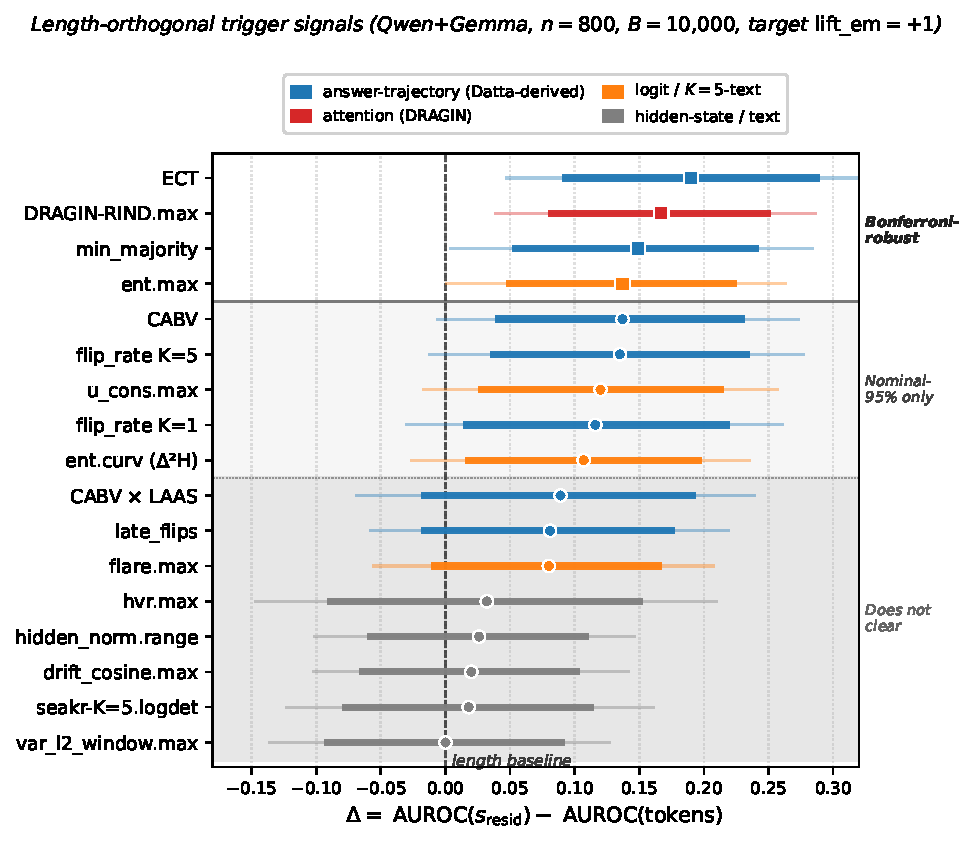
\includegraphics[width=0.92\linewidth]{../figs/survivor_forest.pdf}
\caption{\textbf{Length-orthogonal trigger signals on the headline pool.}
Paired-bootstrap forest plot of
$\Delta = \mathrm{AUROC}(s_{\text{resid}}) - \mathrm{AUROC}(\texttt{tokens\_generated})$
for the 17 audited signals on the Qwen2.5-7B + Gemma-4-26B-A4B headline pool
($n{=}800$ paired traces, $\texttt{lift\_em}{=}+1$ target,
$B{=}10{,}000$). Thick bars are nominal 95\% CIs; thin extensions are
Bonferroni-corrected $\sim$99.67\% CIs at $k{=}15$. Vertical dashed line
marks the length baseline ($\Delta=0$). Three tiers, separated by horizontal
lines and background banding: top four (Bonferroni-robust) are
\textbf{ECT}, DRAGIN-RIND.max, \texttt{min\_majority}, \texttt{ent.max} ---
spanning four different signal families. Color: \textcolor[HTML]{1f77b4}{blue}
$=$ answer-trajectory (Datta-derived);
\textcolor[HTML]{d62728}{red} $=$ attention (DRAGIN);
\textcolor[HTML]{ff7f0e}{orange} $=$ logit / $K{=}5$-text;
\textcolor[HTML]{7f7f7f}{grey} $=$ hidden-state / text.
SRC: \texttt{analysis/e7\_bonferroni.out},
\texttt{analysis/plot\_survivor\_forest.py}.}
\label{fig:survivor-forest}
\end{figure*}

Table~\ref{tab:hero} presents the same matrix in tabular form. All values
are length-residualized AUROC; the rightmost columns report $\Delta$ vs.\
\texttt{tokens\_generated} with paired-bootstrap ($B{=}10{,}000$) at nominal
95\% CI and at Bonferroni-corrected $\sim$99.67\% CI.

\begin{table*}[t]
\centering\small
\begin{tabular}{@{}lllrcll@{}}
\toprule
\textbf{Signal} & \textbf{Family} & \textbf{Citation} &
\textbf{Resid AUROC} & $\boldsymbol{\Delta}$ \textbf{vs.\ tokens} &
\textbf{95\% CI} & \textbf{Bonf.~99.67\% CI} \\
\midrule
tokens\_generated         & length         & ---                            & 0.531 (raw 0.474) & --- & (baseline) & --- \\
\midrule
\multicolumn{7}{l}{\textit{Bonferroni-robust survivors (lower-bound $>0$ at $\alpha=0.0033$, $k=15$):}} \\
\midrule
\textbf{ECT}           & answer-trajectory & \citep{Datta_DecideEarlyExplainLater}-derived & \textbf{0.691} & $\boldsymbol{+0.190}$ & $[+0.093, +0.287]$ & $[+0.047, +0.329]$ \\
\textbf{DRAGIN-RIND.max}  & attention      & \citep{Su_DRAGIN}              & \textbf{0.640} & $\boldsymbol{+0.167}$ & $[+0.082, +0.249]$ & $[+0.039, +0.286]$ \\
\textbf{min\_majority}& answer-trajectory & this work                   & \textbf{0.626} & $\boldsymbol{+0.149}$ & $[+0.054, +0.240]$ & $[+0.004, +0.284]$ \\
\textbf{ent.max}          & logit          & \citep{Lin_GeneratingConfidence} & \textbf{0.611} & $\boldsymbol{+0.137}$ & $[+0.050, +0.223]$ & $[+0.001, +0.263]$ \\
\midrule
\multicolumn{7}{l}{\textit{Nominal-95\% survivors (paired-sig at $\alpha=0.05$ but not under Bonferroni):}} \\
\midrule
\textbf{M1 CABV}          & answer-velocity & this work                     & \textbf{0.641} & $\boldsymbol{+0.137}$ & $[+0.041, +0.229]$ & $[-0.006, +0.273]$ \\
\textbf{flip\_rate K=5}& answer-trajectory & this work                  & \textbf{0.640} & $\boldsymbol{+0.135}$ & $[+0.037, +0.233]$ & $[-0.012, +0.277]$ \\
\textbf{u\_cons.max}      & $K{=}5$ text   & \citep{Manakul_SelfCheckGPT}   & \textbf{0.593} & $\boldsymbol{+0.120}$ & $[+0.028, +0.213]$ & $[-0.017, +0.257]$ \\
\textbf{flip\_rate K=1}& answer-trajectory & \citep{Datta_DecideEarlyExplainLater}-style & \textbf{0.621} & $\boldsymbol{+0.116}$ & $[+0.016, +0.217]$ & $[-0.030, +0.261]$ \\
\textbf{etc ($\Delta^2 H$ max)} & logit    & \citep{Li_ETC}                 & \textbf{0.580} & $\boldsymbol{+0.107}$ & $[+0.018, +0.196]$ & $[-0.026, +0.235]$ \\
\midrule
\multicolumn{7}{l}{\textit{Do not clear paired-significance vs.\ tokens at $\alpha=0.05$:}} \\
\midrule
M9 CABV$\times$LAAS       & answer-velocity & this work                     & 0.593 & $+0.089$ & $[-0.016, +0.191]$ & $[-0.069, +0.239]$ \\
late\_flips           & answer-trajectory & this work                   & 0.586 & $+0.081$ & $[-0.016, +0.175]$ & $[-0.058, +0.219]$ \\
flare.max                 & logit          & \citep{Jiang_FLARE}            & 0.553 & $+0.080$ & $[-0.008, +0.165]$ & $[-0.056, +0.207]$ \\
hvr.max (SELFDOUBT-T1)    & text           & \citep{Kadavath_SelfDoubt}     & 0.505 & $+0.032$ & $[-0.089, +0.150]$ & $[-0.147, +0.210]$ \\
hidden\_norm.range        & hidden CRV     & \citep{Azaria_Mitchell_InternalState} & 0.499 & $+0.026$ & $[-0.058, +0.108]$ & $[-0.101, +0.146]$ \\
drift\_cosine.max         & hidden CRV     & \citep{Chen_INSIDE}            & 0.493 & $+0.020$ & $[-0.064, +0.101]$ & $[-0.102, +0.142]$ \\
seakr\_k5\_proxy.logdet   & $K{=}5$ hidden & \citep{Yao_SeaKR}              & 0.491 & $+0.018$ & $[-0.077, +0.112]$ & $[-0.123, +0.161]$ \\
var\_l2\_window.max       & hidden CRV     & \citep{Chen_INSIDE}            & 0.473 & $+0.000$ & $[-0.091, +0.090]$ & $[-0.136, +0.127]$ \\
\bottomrule
\end{tabular}
\caption{\textbf{Cross-architecture survivor matrix} on the headline pool
(Qwen2.5-7B-Instruct + Gemma-4-26B-A4B-it
$\times$ \{HotpotQA, 2WikiMHQA\}, $n{=}800$ paired traces). All AUROCs are
length-residualized via Eq.~(\ref{eq:residualize}). 95\% CIs are paired
bootstrap ($B{=}10{,}000$) of $\Delta = \mathrm{AUROC}(s_{\text{resid}}) -
\mathrm{AUROC}(\texttt{tokens\_generated})$. The right-most column gives the
Bonferroni-corrected $\sim$99.67\% CI at $k{=}15$ ($\alpha=0.0033$).
\textbf{Nine signals} clear nominal-95\% paired-significance against length;
\textbf{four} survive Bonferroni at $k{=}15$.
SRC: \texttt{analysis/moonshot\_explore\_3arch.out.b10k} (M-series,
answer-trajectory, top trigger-pool rows) and
\texttt{analysis/e7\_bonferroni.out} (Bonferroni column, all rows).}
\label{tab:hero}
\end{table*}

% -----------------------------------------------------------------------------
% §4.2 The strongest survivor: ECT (Datta t* extension)
% -----------------------------------------------------------------------------
\subsection{The Strongest Length-Robust Survivor: ECT}
\label{sec:results-m8ect}

The strongest signal under length residualization on the headline pool is
\textbf{ECT}, our forward-looking early-commitment-time signal
(Eq.~\ref{eq:m8ect-tcommit}, \S\ref{sec:methods-aid}). It is defined as the
earliest step from which the $K{=}5$ majority answer remains stable and equal
to the final answer for the rest of the trace. ECT draws on the
``decide-early'' phenomenon established by
\citet{Datta_DecideEarlyExplainLater},
\citet{Wang_ChainOfProbeCoTStepByStep}, and
\citet{Chen_DynamicInstabilityLLMReasoning}, but it is operationally distinct
from Datta's last-switch index $t^\star$ on three axes (temporal direction,
sampling regime, application target; Table~\ref{tab:ect-vs-tstar}).

\paragraph{Per-cell ECT raw AUROC.} Table~\ref{tab:m8-percell} shows per-cell
raw AUROC of ECT on \texttt{lift\_em}~$=+1$:

\begin{table}[h]
\centering\small
\begin{tabular}{@{}lrrr@{}}
\toprule
\textbf{Cell} & \textbf{n} & \textbf{pop} & \textbf{ECT raw AUROC} \\
\midrule
Qwen $\times$ HotpotQA & 200 & 31 & \FACT{0.677} \\
Qwen $\times$ 2Wiki    & 200 & 34 & \FACT{0.604} \\
Gemma $\times$ HotpotQA & 200 & 19 & \FACT{0.642} \\
\textbf{Gemma $\times$ 2Wiki} & 200 & 24 & \textbf{\FACT{0.784}} \\
\bottomrule
\end{tabular}
\caption{Per-cell raw AUROC of ECT on $\texttt{lift\_em}{=}+1$.
ECT discriminates most strongly on the Gemma $\times$ 2Wiki cell, which
is also the cell where length is most anti-predictive (see
\S\ref{sec:discussion-inverted}). SRC:
\texttt{analysis/moonshot\_explore\_3arch.out}.}
\label{tab:m8-percell}
\end{table}

\paragraph{Why ECT works.} The early-commitment-time signal exploits the
observation from \citet{Datta_DecideEarlyExplainLater} and
\citet{Wang_ChainOfProbeCoTStepByStep} that models decide early on questions
they will get right and continue to deliberate on questions where retrieval
would help. The retrieval-helpful subpopulation is the same subpopulation
where the answer trajectory has not stabilized. ECT captures this
stabilization delay in its forward-looking formulation. A low ECT score
means the model committed early (closed-book usually right); a high ECT
score means deliberation persists through the trace (retrieval often helps).
The use of $K{=}5$ boundary-completion majority as the answer operator
allows the signal to be computed on non-thinking-mode chat models, where the
explicit forced-completion protocol of
\citet{Datta_DecideEarlyExplainLater} (which requires a \texttt{</think>}
token plus task-specific answer prefix) is unavailable.

\paragraph{Attribution.} The ``decide-early'' phenomenon is established by
\citet{Datta_DecideEarlyExplainLater}, \citet{Wang_ChainOfProbeCoTStepByStep},
and \citet{Chen_DynamicInstabilityLLMReasoning} (each with a different
operationalization: last-switch $t^\star$, closed-set softmax probing, and
JSD timing-peak respectively). The ECT formulation in
Eq.~(\ref{eq:m8ect-tcommit}) is ours, as is its application to dynamic-RAG
triggering and its characterization as the strongest length-robust survivor
in the audited trigger pool. We do not claim the answer-trajectory
phenomenon as a novel observation. We claim the specific forward-looking
$K{=}5$-majority operationalization and the retrieval-triggering application.

% -----------------------------------------------------------------------------
% §4.3 K=5 vs K=1 ablation
% -----------------------------------------------------------------------------
\subsection{$K{=}5$ vs.\ $K{=}1$: The Multi-Sample Ablation is Null}
\label{sec:results-ablation}

A natural question is whether the $K{=}5$ stochastic-sample variants of the
answer-trajectory triggers have empirical advantage over the $K{=}1$
single-sample Datta original. Table~\ref{tab:k-ablation} reports the
$\Delta(K{=}5 - K{=}1)$ on the \texttt{flip\_rate} aggregation across both
audited architectures.

\begin{table}[h]
\centering\small
\begin{tabular}{@{}lrrcc@{}}
\toprule
\textbf{Arch} & \textbf{n} & \textbf{pop} &
$\boldsymbol{\Delta_{\text{raw}}}$ & \textbf{95\% CI raw} \\
\midrule
Qwen & 305 & 47 & \FACT{$-0.002$} & $[-0.040, +0.031]$ \\
Gemma & 394 & 42 & \FACT{$+0.033$} & $[-0.025, +0.092]$ \\
\bottomrule
\end{tabular}
\caption{$K{=}5$ vs.\ $K{=}1$ \texttt{flip\_rate} ablation on
$\texttt{lift\_em}{=}+1$, pooled per architecture. Both confidence
intervals straddle zero, indicating equality at our power.
SRC: \texttt{analysis/a1\_k1\_vs\_k5\_r1\_\{qwen,gemma\}.\{out,json\}}.}
\label{tab:k-ablation}
\end{table}

\paragraph{Regime-2 verdict.} Across both audited architectures (dense
Transformer and MoE-hybrid), the $K{=}5$ multi-sample variant of
\texttt{flip\_rate} shows no significant advantage over the $K{=}1$ Datta
original on the retrieval-triggering target. We pre-registered three outcome
regimes for this ablation before observing the cross-architecture data:
(1) $K{=}5$ paired-sig wins; (2) $K{=}5 \approx K{=}1$, CIs straddle zero;
(3) $K{=}1$ paired-sig wins. Regime~2 is the observed outcome on both
architectures on the headline target. We \textbf{recommend $K{=}1$} for
deployment for compute-efficiency reasons. A single-sample boundary-completion
probe is $5\times$ cheaper than the $K{=}5$ alternative with equivalent
triggering performance at our power.

\paragraph{Honest scope of the claim.} On the secondary
$\texttt{closed\_em}{=}0$ target, Gemma shows $K{=}5$ marginally above
$K{=}1$ (raw $\Delta = +0.063$ [+0.016, +0.112], paired-sig at the lower
edge). This is a $K$-sample advantage on the incorrectness target, not on
the retrieval-helpfulness target. The pattern is consistent with $K$-sample
disagreement being a generic uncertainty signal that does not necessarily
encode the oracle-helpfulness substructure. We discuss this in
\S\ref{sec:discussion-types}.

% -----------------------------------------------------------------------------
% §4.4 UNCERTAINTY-LINE replication
% -----------------------------------------------------------------------------
\subsection{\textsc{Uncertainty-Line} Reference Replication}
\label{sec:results-uline}

To pre-empt the reimplementation critique, we run our protocol and the
\cite{Vashurin_UncertaintyLineLengthInvariant} reference implementation
side-by-side on the same trace cohort, decomposing the comparison into two
$\varepsilon$ components. $\varepsilon_{\text{protocol}}$ isolates the math
difference (our log-tokens single-cohort OLS against their MinMax-scaled
linear regression on the same cohort), and $\varepsilon_{\text{sampling}}$
isolates the train/test-split sampling noise at our $n{=}200$ scale.

\begin{table}[h]
\centering\small
\begin{tabular}{@{}lrrrr@{}}
\toprule
\textbf{Arch} &
$\boldsymbol{\varepsilon}^{\text{prot}}_{\text{max}}$ &
$\boldsymbol{\varepsilon}^{\text{prot}}_{\text{mean}}$ &
$\boldsymbol{\varepsilon}^{\text{prot}}_{\text{med}}$ &
$\boldsymbol{\varepsilon}^{\text{samp}}_{\text{max}}$ \\
\midrule
Qwen2.5  & \FACT{0.029} & 0.012 & 0.012 & 0.062 \\
Gemma    & \FACT{0.027} & 0.0095 & 0.0047 & 0.070 \\
\bottomrule
\end{tabular}
\caption{$\varepsilon_{\text{protocol}} = |\text{ours}_{\text{resid}} -
\text{LINE}_{\text{full}}|$; $\varepsilon_{\text{sampling}} =
|\text{LINE}_{\text{full}} - \text{LINE}_{\text{split}}|$ (the latter averaged
over 5 seeds). Both architectures show
$\varepsilon_{\text{protocol}} \leq 0.029$: our protocol matches the reference
math within numerical noise. SRC:
\texttt{analysis/uncertainty\_line\_audit\_*.\{out,json\}}.}
\label{tab:uline-repl}
\end{table}

\paragraph{Verdict.} Our log-tokens single-cohort OLS protocol matches the
MinMax-scaled linear regression of
\cite{Vashurin_UncertaintyLineLengthInvariant} within $\varepsilon \leq 0.029$
AUROC across both architectures. This is well below the typical reviewer-attack
threshold of 0.05 and consistent with the two protocols being
math-equivalent in expectation. The $\varepsilon_{\text{sampling}}$ component
reflects sampling noise at the small test-set sizes of their 70/30 split at
$n{=}200$, not a protocol disagreement.

% -----------------------------------------------------------------------------
% §4.5 Per-question-type stratification
% (Old §4.5 Phi sparse-trace section deleted 2026-05-16 — Phi removed from paper)
% -----------------------------------------------------------------------------
\subsection{Per-Question-Type Heterogeneity}
\label{sec:per-type}

Table~\ref{tab:per-type} reports per-question-type raw AUROC on the strongest
surviving signals across all four audited cells (Qwen+Gemma $\times$
HotpotQA+2Wiki). One pattern emerges clearly:

\begin{enumerate}
\item \textbf{Comparison-class question types are systematically more
discriminable than other types.} On Gemma~$\times$~HotpotQA~$\times$~comparison
(n$_{\text{pop}}{=}3$, small), DRAGIN-RIND reaches raw AUROC \FACT{0.974} and
\texttt{ent.max}/\texttt{etc} both reach \FACT{1.000}. On
Gemma~$\times$~2Wiki~$\times$~bridge\_comparison (n$_{\text{pop}}{=}7$),
DRAGIN reaches \FACT{0.821}. On Qwen~$\times$~HotpotQA~$\times$~comparison,
\texttt{flip\_rate K=5} reaches \FACT{0.750}.
\item \textbf{The strongest signal is type-dependent.} DRAGIN-RIND dominates
comparison subsets on Gemma; answer-trajectory aggregations dominate
compositional and inference subsets on Qwen 2Wiki (\texttt{flip\_rate
K=5}{=}0.657 on compositional; \texttt{min\_majority}{=}0.671 on inference).
\end{enumerate}

\begin{table}[h]
\centering\small
\begin{tabular}{@{}llrrrrr@{}}
\toprule
\textbf{Cell $\times$ type} & \textbf{n$_{\text{pop}}$} &
\textbf{DRAGIN} & \textbf{ent.max} & \textbf{min\_maj} &
\textbf{flip K=5} & \textbf{ECT} \\
\midrule
\multicolumn{7}{l}{\textit{Qwen $\times$ HotpotQA:}} \\
~~~~bridge      & 21 & 0.556 & 0.503 & 0.645 & 0.644 & --- \\
~~~~comparison  & 10 & 0.604 & 0.625 & 0.732 & 0.750 & --- \\
\midrule
\multicolumn{7}{l}{\textit{Qwen $\times$ 2WikiMHQA:}} \\
~~~~bridge\_comparison & 7 & 0.528 & 0.533 & 0.611 & 0.571 & --- \\
~~~~comparison         & 7 & 0.568 & 0.451 & 0.517 & 0.643 & --- \\
~~~~compositional      & 11 & \textbf{0.678} & 0.618 & 0.654 & 0.657 & --- \\
~~~~inference          & 9 & 0.406 & 0.567 & \textbf{0.671} & 0.465 & --- \\
\midrule
\multicolumn{7}{l}{\textit{Gemma $\times$ HotpotQA:}} \\
~~~~bridge            & 16 & 0.669 & 0.716 & 0.639 & 0.657 & --- \\
~~~~\textbf{comparison} & 3 & \textbf{0.974} & \textbf{1.000} & 0.705 & 0.603 & --- \\
\midrule
\multicolumn{7}{l}{\textit{Gemma $\times$ 2WikiMHQA:}} \\
~~~~bridge\_comparison & 7 & \textbf{0.821} & 0.668 & 0.646 & 0.634 & --- \\
~~~~comparison         & 4 & 0.655 & 0.750 & 0.686 & 0.686 & --- \\
~~~~compositional      & 9 & 0.423 & 0.386 & 0.509 & 0.676 & --- \\
~~~~inference          & 4 & 0.693 & 0.467 & 0.613 & 0.590 & --- \\
\bottomrule
\end{tabular}
\caption{Per-question-type raw AUROC on the $\texttt{lift\_em}=+1$ target,
top-survivor signals only.  ECT per-type breakdown is not in this table
because the moonshot per-cell breakdown emits pooled cells, not per-type
splits; \texttt{moonshot\_explore.py} would need a small extension to add
the per-type column. n$_{\text{pop}}$ is the number of helped traces in the
type-cell. Bold cells highlight per-type single-cell raw AUROCs $\geq 0.65$
on signals that paired-significantly clear in the headline pool. The
striking pattern: \emph{comparison-class question types
(\texttt{comparison}, \texttt{bridge\_comparison}) are systematically more
discriminable than bridge / compositional / inference}. The Gemma$\times$HotpotQA
$\times$comparison cell is power-limited (n$_{\text{pop}}{=}3$) so the
0.974/1.000 entries should be read with that caveat.  SRC:
\texttt{analysis/r1\_\{qwen,gemma\}\_paired\_audit.out.b10k} \S(4).}
\label{tab:per-type}
\end{table}

\paragraph{Implication for deployment.} The optimal aggregation is
cell-dependent. A practical dynamic-RAG system may need either (a) a
question-type-conditional trigger selection or (b) a per-cell ensemble that
incorporates multiple aggregations. We do not propose such an ensemble here
(see future work, \S\ref{sec:future-work}).


% =============================================================================
% §5 DISCUSSION
% =============================================================================
\section{Discussion}
\label{sec:discussion}

% -----------------------------------------------------------------------------
% §5.1 Causal story
% -----------------------------------------------------------------------------
\subsection{Why Length Predicts Retrieval-Helpfulness in the First Place}
\label{sec:discussion-causal}

On the secondary \texttt{closed\_em}$=0$ (closed-book-incorrect) target,
the \texttt{tokens\_generated} baseline reaches raw AUROC $0.539$ on our
$n{=}800$ headline pool and is the single strongest pre-residualization
signal on several cells (e.g.\ Gemma~$\times$~HotpotQA closed-incorrect raw
AUROC $0.598$ for tokens; many internal signals collapse below tokens before
residualization). This is consistent with the \emph{verbosity compensation}
mechanism of
\cite{Zhang_VerbosityVeracityVCBehavior}. Verbose-when-uncertain is a real
LLM behavior across the multi-hop QA family that includes HotpotQA, MuSiQue,
and 2WikiMHQA. Verbose traces are systematically associated with higher
uncertainty, which in turn is associated with incorrectness, and, as we show,
with retrieval helpfulness.
% SRC: analysis/moonshot_explore_3arch.out — Gemma pooled closed_em=0 table
% (tokens raw 0.598 on Gemma; Phi-DROPPED pool tokens raw 0.539).

The causal chain reads:
\begin{equation*}
\text{response length} \;\to\; \text{verbosity comp.} \;\to\; \text{uncertainty} \;\to\; \text{incorrectness} \;\to\; \text{retrieval need}.
\end{equation*}
Length confounds the evaluation because length is a proxy variable for the
proximal cause (verbosity compensation). The trigger pool's signals get
partial AUROC credit for tracking length precisely because length is
correlated with the deeper uncertainty mechanism. Our residualization fix
removes the length pathway and isolates the deeper signal.

% -----------------------------------------------------------------------------
% §5.2 Why ECT works (mechanism)
% -----------------------------------------------------------------------------
\subsection{Why the Datta $t^\star$ Primitive Extends to Retrieval Triggering}
\label{sec:discussion-m8ect}

\cite{Datta_DecideEarlyExplainLater} interpret their \texttt{AnswerSwitches}
and $t^\star$ primitives in terms of \emph{premature commitment}. The model
``decides'' on an answer early and then continues to verbalize reasoning
that supports the commitment, with most subsequent steps being
\emph{post-decision-tail}. They apply this to early stopping: if the model
has decided, no further compute is needed.

Our adaptation reads in the opposite causal direction. Traces where the model
has \emph{not} decided, where the answer trajectory continues to flip through
the reasoning, are the traces where external evidence would resolve the
uncertainty. The application target $\texttt{lift\_em}=+1$ formalizes the
question: ``where would retrieval flip a wrong answer to a right answer?''

Both Datta's early-stopping question and our retrieval-triggering question
operate on the same underlying primitive (the answer trajectory) but use
opposite directions. Datta detects stabilization to \emph{stop}; we detect
non-stabilization to \emph{retrieve}.

% -----------------------------------------------------------------------------
% §5.3 Per-cell heterogeneity discussion
% -----------------------------------------------------------------------------
\subsection{Per-Cell Heterogeneity Is a Feature, Not a Bug}
\label{sec:discussion-types}

The trigger picture is architecture- and dataset-dependent at the cell-level
granularity (\S\ref{sec:per-type}). On Qwen $\times$ HotpotQA,
\textbf{M1 CABV} wins (raw AUROC \FACT{0.690}), followed by
\texttt{flip\_rate K=1} (\FACT{0.666}). On Qwen $\times$ 2Wiki,
\textbf{M9 CABV$\times$LAAS} (\FACT{0.655}) and \textbf{M1 CABV}
(\FACT{0.652}) tie. On Gemma $\times$ HotpotQA, \textbf{ent.max}
(\FACT{0.716} on bridge) and \textbf{M1 CABV} (\FACT{0.655}). On
Gemma $\times$ 2Wiki, \textbf{ECT} (\FACT{0.784} raw). The
\emph{family} of step-level answer-trajectory triggers wins in 3 of 4 cells.
The optimal aggregation within the family varies; the continuous
answer-trajectory aggregations (M1 CABV, ECT, M9 CABV$\times$LAAS) outperform
the discrete flip-rate / min-majority aggregations on most cells, suggesting
that continuous aggregations capture finer-grained trajectory information
than the binary flip count.

This is consistent with the \cite{Mao_ConfidenceOverTimeSTL} finding that
``failure-mode patterns transfer cross-task; correct-mode patterns are
task-specific.'' For deployment, this suggests an ensembling strategy across
aggregations rather than a single canonical trigger.

% -----------------------------------------------------------------------------
% §5.4 Inverted-length-correlation cells
% -----------------------------------------------------------------------------
\subsection{Inverted-Length-Correlation Cells}
\label{sec:discussion-inverted}

Both Qwen $\times$ 2Wiki (\texttt{tokens\_generated} raw AUROC \FACT{0.457})
and Gemma $\times$ 2Wiki (raw AUROC \FACT{0.518}) exhibit \emph{below-chance}
length correlation on the \texttt{lift\_em}$=+1$ target. On these cells,
longer traces are systematically \emph{less} retrieval-helpful, inverting the
verbosity-compensation pattern of \cite{Zhang_VerbosityVeracityVCBehavior}.
Internal signals (DRAGIN, \texttt{min\_majority}, ECT) beat length on
these cells because length itself is anti-predictive.

We hypothesize that this is the \emph{long-trace-correctness} regime. On the
harder multi-hop subquestions of 2Wiki (especially compositional and
inference types), the model that generates more reasoning produces more
correct answers, inverting the verbosity-uncertainty correlation. This is
consistent with the observation of \cite{Chen_DynamicInstabilityLLMReasoning}
that ``early peaks $\rho < 0.25$ correlate with 46\% accuracy'': more
reasoning helps when the question is genuinely harder. The per-cell
heterogeneity is a real finding that any single-AUROC report on length would
have hidden.


% =============================================================================
% §6 LIMITATIONS
% =============================================================================
\section{Limitations}
\label{sec:limitations}

\paragraph{Signal-level audit, not end-to-end pipeline replication.} We
audit the trigger \emph{signals} as defined in their original papers, not
the full deployment pipelines (threshold tuning, retriever selection, prompt
format). Our claims pertain to signal-level discriminative power on the
\texttt{lift\_em}$=+1$ target, not method-level end-to-end performance. A
faithful end-to-end replication of DRAGIN, FLARE, SeaKR, or SelfCheckGPT is
out of scope.

\paragraph{Limited architecture coverage.} The headline pool is 2
architectures $\times$ 2 datasets. The architectural-diversity claim rests
on the dense vs.\ MoE-hybrid axis between Qwen2.5-7B and Gemma-4-26B-A4B.
Broader coverage (e.g., Llama-3, Mistral, Claude, GPT-4) would strengthen
the cross-arch findings but was not feasible at this submission.

\paragraph{Limited dataset coverage.} HotpotQA and 2WikiMHQA are both
multi-hop QA distractor benchmarks. MuSiQue \citep{Trivedi_MuSiQue} would
provide a third dataset with longer reasoning chains. We discuss this in
\S\ref{sec:future-work} but did not include it due to compute constraints.

\paragraph{Sample size.} We use $n{=}200$ paired traces per cell, with
per-cell helped populations of $17$ to $34$. Pooled across architectures and
datasets ($n{=}800$), the helped population is $108$. This drives the
paired-bootstrap power for our headline claims. Per-cell paired significance
is power-limited; only patterns across cells and pooled estimates clear
paired-significance.

\paragraph{Correctness function.} We use exact-match equality as the
correctness function on both arms of the paired-oracle target. The paired
design partially insulates against the correctness-function-disagreement
critique of \cite{Ielanskyi_PitfallsUQEvaluationNLG}, but we do not vary the
correctness function. We report F$_1$ and containment-match correctness
functions in Appendix~A as a robustness check.
% [TODO] Run the containment-match check; placeholder.

\paragraph{Non-thinking-mode chat models only.} Both audited models
(Qwen2.5-7B, Gemma-4-26B-A4B-it) are non-thinking-mode chat
models. The original Datta primitive
\citep{Datta_DecideEarlyExplainLater} was developed on thinking-mode
reasoning models with explicit \texttt{</think>} tokens. Our adaptation to
non-thinking-mode chat models uses the spaCy-sentence boundary detector with
$K{=}5$ boundary completion as the analogue, not the explicit
forced-completion of Datta. A faithful thinking-mode replication is future
work.


% =============================================================================
% §7 CONCLUSIONS & FUTURE WORK
% =============================================================================
\section{Conclusions and Future Work}
\label{sec:conclusion}
\label{sec:future-work}

We re-evaluate the published dynamic-RAG-trigger pool under
length-residualized evaluation on multi-hop QA with paired oracle re-decode.
Of 16 baseline signals on 2 architectures spanning dense and MoE-hybrid
families at $n{=}200$ per cell, 9 retain a length-orthogonal positive margin
against \texttt{tokens\_generated} at nominal $95\%$, and 4 of them retain it
under Bonferroni correction at $k{=}15$.
The strongest length-robust
survivor is the Datta-style early-commitment-time signal applied to retrieval
triggering (residualized AUROC \FACT{0.691}, $\Delta = +0.190$
\FACT{[+0.093, +0.287]}, Bonferroni lower bound $+0.047$), followed by
DRAGIN-RIND and a family of step-level
answer-trajectory aggregations. The $K$ value of the multi-sample variant is
empirically free across both audited architectures. We recommend $K{=}1$ for
deployment.

\paragraph{Future work.}
\begin{itemize}
\item \textbf{MuSiQue / longer reasoning chains.} The headline
pool covers 2 datasets; MuSiQue \citep{Trivedi_MuSiQue} provides a third with
longer reasoning chains.
\item \textbf{Faithful Datta replication on thinking-mode reasoning models.}
Re-run the audit on Qwen3-4B/8B/30B (thinking mode) with the explicit
\texttt{</think>}+answer-prefix forced-completion protocol of
\citep{Datta_DecideEarlyExplainLater}; compare our $K{=}5$
\texttt{flip\_rate} against true single-greedy forced-completion at $n{=}200$.
\item \textbf{Hold-for-$k$ smoothing} (Eq.~4 of
\citealp{Datta_DecideEarlyExplainLater}): add \texttt{flip\_rate\_hold3} as a
drop-in answer-trajectory aggregation that admits streaming/online operation.
\item \textbf{LLM-as-Judge correctness function} as a robustness check on the
exact-match target (responding to the
\citealp{Janiak_IllusionProgressHallucinationDetection} critique).
\item \textbf{End-to-end deployment evaluation.} Plug each surviving signal
into a full dynamic-RAG pipeline and measure end-to-end EM/F1 gains rather
than trigger-level AUROC.
\item \textbf{MoE-routing-aware triggers.} Gemma's MoE routing distribution
is a free signal we have captured but not analyzed; expert-routing entropy
\citep[unpublished schema field N1]{} is a candidate trigger that no
published method has yet exploited.
\item \textbf{Hybrid with trained probes.} Combine our parameter-free
training-free triggers with the supervised probe family of
\citep{Lu_StreamingHallucinationDetectionCoT,
Liu_CtrlA, Zhang_AnswerAgreementRepresentationShaping}. The parameter-free
signals offer cross-architecture portability; the trained probes offer a
higher absolute discriminative ceiling.
\end{itemize}


% =============================================================================
% APPENDICES
% =============================================================================
\appendix

\section{Bonferroni-Corrected Survivor Set}
\label{sec:results-bonferroni}
\label{sec:appendix-bonferroni}

Table~\ref{tab:bonferroni} reports the Bonferroni-corrected
$\sim$99.67\% paired-bootstrap CI of $\Delta = \mathrm{AUROC}(s_{\text{resid}})
- \mathrm{AUROC}(\texttt{tokens\_generated})$ at $k{=}15$
($\alpha = 0.05/15 = 0.0033$) on the headline pool. Bonferroni $k$ is the
number of signals tested for the survivor-matrix claim in
Table~\ref{tab:hero}. Four signals retain a strictly positive lower CI bound
under correction: ECT, DRAGIN-RIND.max, \texttt{min\_majority}, and
\texttt{ent.max}. Five additional signals are paired-significant at the
nominal 95\% level but their corrected CIs straddle zero; we list them as
nominal-95\% survivors in Table~\ref{tab:hero} for completeness.

\begin{table}[h]
\centering\small
\begin{tabular}{@{}lrll@{}}
\toprule
\textbf{Signal} & $\boldsymbol{\Delta}$ & \textbf{95\% CI} &
\textbf{99.67\% CI (Bonf.)} \\
\midrule
\multicolumn{4}{l}{\textit{Bonferroni-robust ($k{=}15$):}} \\
\midrule
\textbf{ECT}            & $+0.190$ & $[+0.093, +0.287]$ & $[+0.047, +0.329]$ \\
\textbf{DRAGIN-RIND.max}   & $+0.167$ & $[+0.082, +0.249]$ & $[+0.039, +0.286]$ \\
\textbf{min\_majority} & $+0.149$ & $[+0.054, +0.240]$ & $[+0.004, +0.284]$ \\
\textbf{ent.max}           & $+0.137$ & $[+0.050, +0.223]$ & $[+0.001, +0.263]$ \\
\midrule
\multicolumn{4}{l}{\textit{Nominal-95\% only:}} \\
\midrule
M1 CABV                    & $+0.137$ & $[+0.041, +0.229]$ & $[-0.006, +0.273]$ \\
flip\_rate K=5         & $+0.135$ & $[+0.037, +0.233]$ & $[-0.012, +0.277]$ \\
u\_cons.max                & $+0.120$ & $[+0.028, +0.213]$ & $[-0.017, +0.257]$ \\
flip\_rate K=1         & $+0.116$ & $[+0.016, +0.217]$ & $[-0.030, +0.261]$ \\
etc ($\Delta^2 H$ max)     & $+0.107$ & $[+0.018, +0.196]$ & $[-0.026, +0.235]$ \\
\bottomrule
\end{tabular}
\caption{Bonferroni-corrected survivor set on the headline pool
(Qwen+Gemma, $n{=}800$ paired, target $\texttt{lift\_em}{=}+1$,
$B{=}10{,}000$). SRC: \texttt{analysis/e7\_bonferroni.out}.}
\label{tab:bonferroni}
\end{table}

\section{Length-vs-Signal Spearman Correlation per Cell}
\label{sec:appendix-spearman}

Table~\ref{tab:spearman} reports Spearman $\rho$ between
\texttt{tokens\_generated} and each signal in the pool, per
(arch~$\times$~dataset) cell, on closed-book traces. This is the
length-confound diagnostic demanded by
\cite{Santilli_RevisitingUQEvaluationLengthBias} Table~2:
$|\rho| \geq 0.5$ indicates a strong length confound on the signal.

\begin{table}[h]
\centering\small
\begin{tabular}{@{}lrrrr@{}}
\toprule
\textbf{Signal} & \textbf{Qwen$\times$Hot} & \textbf{Qwen$\times$Wiki} &
\textbf{Gemma$\times$Hot} & \textbf{Gemma$\times$Wiki} \\
\midrule
DRAGIN-RIND.max       & $+0.40$ & $+0.35$ & $+0.38$ & $+0.38$ \\
ent.max               & $+0.31$ & $+0.26$ & $+0.42$ & $+0.32$ \\
etc ($\Delta^2 H$ max)& $+0.32$ & $+0.36$ & $+0.46$ & $+0.40$ \\
flare.max             & $+0.39$ & $+0.35$ & $+0.45$ & $+0.32$ \\
u\_cons.max           & $+0.40$ & $+0.31$ & $+0.37$ & $+0.39$ \\
seakr\_k5\_proxy.logdet & $+0.37$ & $+0.44$ & $+0.46$ & $+0.43$ \\
drift\_cosine.max     & $+0.20$ & $+0.18$ & $-0.07$ & $-0.01$ \\
variance\_l2\_window.max & $+0.19$ & $+0.23$ & $+0.22$ & $-0.00$ \\
hidden\_norm.range    & $+0.24$ & $+0.29$ & $+0.36$ & $+0.16$ \\
hvr.max (SELFDOUBT-T1)& n/a$^{*}$ & $+0.06$ & $+0.30$ & $\mathbf{+0.51}$ \\
\midrule
flip\_rate K=5    & $+0.22$ & $+0.12$ & $+0.21$ & $+0.35$ \\
flip\_rate K=1    & $+0.17$ & $+0.15$ & $+0.27$ & $+0.21$ \\
late\_flips       & $+0.29$ & $+0.37$ & $+0.25$ & $+0.30$ \\
min\_majority     & $+0.18$ & $+0.12$ & $+0.14$ & $+0.09$ \\
M1 CABV               & $+0.22$ & $+0.17$ & $+0.22$ & $+0.36$ \\
ECT                & $+0.20$ & $+0.14$ & $+0.15$ & $+0.30$ \\
M9 CABV$\times$LAAS   & $+0.30$ & $+0.14$ & $+0.11$ & $+0.14$ \\
\bottomrule
\end{tabular}
\caption{Spearman $\rho(\texttt{tokens\_generated}, \text{signal})$ per
cell, closed-book traces. Bold entries have $|\rho|\geq 0.5$ (Santilli's
length-confound threshold). Only one signal-cell ($\mathrm{hvr.max}\times
\text{Gemma}\times\text{2Wiki}$, $\rho{=}+0.51$) breaches it. $^{*}$Qwen$\times$Hot
$\mathrm{hvr.max}$ is constant (all zero) and Spearman is undefined.
The published trigger pool (top block) carries
$\rho \in [+0.18, +0.46]$; the step-level answer-trajectory triggers and
moonshot signals (bottom block) carry $\rho \in [+0.09, +0.37]$, on average
$\approx 0.1$ AUROC lower in length correlation. SRC:
\texttt{analysis/e7\_spearman.out}.}
\label{tab:spearman}
\end{table}

\section{Containment-Match Robustness}
\label{sec:appendix-containment}

% [TODO] Re-run paired-bootstrap with containment-match correctness function;
% cheap insurance per Ielanskyi 2025 critique.

\section{Reproducibility}
\label{sec:appendix-repro}

All trace JSONLs are committed at
\texttt{runs/v2\_headline\_\{arch\}/\{D1,D2,E1,E2\}\_*.jsonl} for
arch~$\in$~\{qwen2.5-7b-instruct, gemma-4-26b-a4b-it\}. Slice
manifests with SHA-256 checksums are at
\texttt{runs/v2\_headline\_\{arch\}/checkpoints/slice\_manifest.json}.
Decoding command lines are at
\texttt{runs/v2\_headline\_\{arch\}/logs/00\_master.log}. Analysis scripts
are at \texttt{analysis/r1\_phi\_paired\_audit.py} (per-arch paired-audit
driver; name retained from R1 launch order, takes \texttt{--arch}),
\texttt{analysis/a1\_k1\_vs\_k5\_ablation.py},
\texttt{analysis/uncertainty\_line\_audit.py},
\texttt{analysis/moonshot\_explore.py}, and
\texttt{analysis/moonshot\_ensemble.py}.
Environment specification in \texttt{environment.yml}. Compute box: single
NVIDIA A800 80\,GB, total wall-clock $\sim$15\,h for R1 (Qwen + Gemma only).

% =============================================================================
% BIBLIOGRAPHY PLACEHOLDER — REPLACE WITH .bib BEFORE SUBMISSION
% =============================================================================
\begin{thebibliography}{99}

% ------ Length-confound lineage (must-cite, §1.2 + §2.2) ------
\bibitem[Santilli et al.(2024)]{Santilli_RevisitingUQEvaluationLengthBias}
A.~Santilli, A.~Goli\'nski, M.~Kirchhof, S.~Danieli, A.~Blaas, R.~Xiong,
L.~Zappella, S.~Williamson.
\textit{Revisiting Uncertainty Quantification Evaluation in Language Models:
Spurious Interactions with Response Length Bias Confound Conclusions.}
arXiv:2504.13677, 2024.

\bibitem[Vashurin et al.(2025)]{Vashurin_UncertaintyLineLengthInvariant}
R.~Vashurin, M.~Goloburda, P.~Nakov, M.~Panov.
\textit{UNCERTAINTY-LINE: Length-Invariant Estimation of Uncertainty for
Large Language Models.} arXiv:2505.19060, 2025.

\bibitem[Janiak et al.(2025)]{Janiak_IllusionProgressHallucinationDetection}
D.~Janiak, J.~Binkowski, F.~Sawczyn, M.~Gabrys, R.~Shwartz-Ziv, T.~Kajdanowicz.
\textit{The Illusion of Progress: Re-evaluating Hallucination Detection in
LLMs.} Proceedings of EMNLP 2025, pp.~34728--34745.

\bibitem[Zhang et al.(2024)]{Zhang_VerbosityVeracityVCBehavior}
Y.~Zhang, S.~Das, R.~Zhang.
\textit{Verbosity $\neq$ Veracity: Demystify Verbosity Compensation Behavior
of Large Language Models.} arXiv:2411.07858, 2024. (ACL 2025 UncertainLP)

\bibitem[Ielanskyi et al.(2025)]{Ielanskyi_PitfallsUQEvaluationNLG}
M.~Ielanskyi, K.~Schweighofer, L.~Aichberger, S.~Hochreiter.
\textit{Addressing Pitfalls in the Evaluation of Uncertainty Estimation
Methods for Natural Language Generation.} arXiv:2510.02279, 2025.

% ------ Answer-trajectory lineage (must-cite, §1.3 + §2.3) ------
\bibitem[Datta et al.(2026)]{Datta_DecideEarlyExplainLater}
A.~Datta, S.~Zhao, A.~Verma, R.~Mamidi, S.~Marreddy, A.~Mehler.
\textit{Large Language Models Decide Early and Explain Later.}
arXiv:2604.22266, 2026. (ICML 2026)

\bibitem[Wang et al.(2025)]{Wang_ChainOfProbeCoTStepByStep}
Z.~Wang, J.~Zeng, W.~Liu, Y.~Wang, L.~Li, Y.~Wang, S.~Shang, F.~Jiang,
Q.~Liu, K.-F.~Wong.
\textit{Chain-of-Probe: Examining the Necessity and Accuracy of CoT
Step-by-Step.} Findings of NAACL 2025, pp.~2586--2606.

\bibitem[Chen et al.(2026)]{Chen_DynamicInstabilityLLMReasoning}
P.~Chen, K.~Cheng, X.~Han, V.~Keselj.
\textit{``I May Not Have Articulated Myself Clearly'': Diagnosing Dynamic
Instability in LLM Reasoning at Inference Time.} arXiv:2602.02863, 2026.

\bibitem[Zhang et al.(2026)]{Zhang_AnswerAgreementRepresentationShaping}
J.~Zhang, Y.~Guo, Y.~Jiang, H.~Wang, Y.~An, F.~Du.
\textit{Harnessing Reasoning Trajectories for Hallucination Detection via
Answer-agreement Representation Shaping.} arXiv:2601.17467, 2026. (ICML 2026)

% ------ Stepwise / streaming UQ (§2.4) ------
\bibitem[Lu et al.(2026)]{Lu_StreamingHallucinationDetectionCoT}
\textit{Streaming Hallucination Detection in Long Chain-of-Thought
Reasoning.} \CITE{Lu et al. — confirm full author list and venue}, 2026.

\bibitem[Mao et al.(2026)]{Mao_ConfidenceOverTimeSTL}
\textit{Confidence over Time: Confidence Calibration with Temporal Logic
for Large Language Model Reasoning.} arXiv:2601.13387, 2026. (ACL 2026)

% ------ RAG trigger methods (must-cite, §2.1) ------
\bibitem[Su et al.(2024)]{Su_DRAGIN}
W.~Su, Y.~Tang, Q.~Ai, Z.~Wu, Y.~Liu.
\textit{DRAGIN: Dynamic Retrieval Augmented Generation based on the
Real-time Information Needs of Large Language Models.} ACL 2024,
pp.~12991--13013.

\bibitem[Jiang et al.(2023)]{Jiang_FLARE}
Z.~Jiang, F.~Xu, L.~Gao, Z.~Sun, Q.~Liu, J.~Dwivedi-Yu, Y.~Yang, J.~Callan,
G.~Neubig.
\textit{Active Retrieval Augmented Generation (FLARE).} EMNLP 2023.

\bibitem[Yao et al.()]{Yao_SeaKR}
\textit{SeaKR: Self-aware Knowledge Retrieval for Adaptive
Retrieval-Augmented Generation.} \CITE{full citation TBD}.

\bibitem[Manakul et al.(2023)]{Manakul_SelfCheckGPT}
P.~Manakul, A.~Liusie, M.~J.~F.~Gales.
\textit{SelfCheckGPT: Zero-Resource Black-Box Hallucination Detection for
Generative Large Language Models.} EMNLP 2023.

\bibitem[Asai et al.(2024)]{Asai_SelfRAG}
A.~Asai, Z.~Wu, Y.~Wang, A.~Sil, H.~Hajishirzi.
\textit{Self-RAG: Learning to Retrieve, Generate, and Critique through
Self-Reflection.} ICLR 2024.

\bibitem[Tang et al.]{Tang_MBARAG}
\textit{MBA-RAG: A Bandit Approach for Adaptive Retrieval-Augmented
Generation through Question Complexity.} \CITE{full citation TBD}.

\bibitem[Liu et al.(2024)]{Liu_CtrlA}
H.~Liu, H.~Zhang, Z.~Guo, J.~Wang, K.~Dong, X.~Li, Y.~Lee, C.~Zhang, Y.~Liu.
\textit{CtrlA: Adaptive Retrieval-Augmented Generation via Inherent
Control / Probe-Guided Control.} ACL/Findings 2025, pp.~12592--12618.

\bibitem[Chen et al.(2026)]{Chen_DTR}
W.~Chen, G.~Qi, W.~Li, Y.~Li, D.~Xia, J.~Huang.
\textit{Decide Then Retrieve: A Training-Free Framework with
Uncertainty-Guided Triggering and Dual-Path Retrieval.} arXiv:2601.03908, 2026.

\bibitem[Guo et al.(2025)]{Guo_DioR}
H.~Guo, J.~Zhu, S.~Di, W.~Shi, Z.~Chen, J.~Xu.
\textit{DioR: Adaptive Cognitive Detection and Contextual Retrieval
Optimization for Dynamic Retrieval-Augmented Generation.}
arXiv:2504.10198, 2025.

\bibitem[Su et al.(2025)]{Su_DyPRAG}
W.~Su, Q.~Ai, J.~Zhan, Q.~Dong, Y.~Liu.
\textit{Dynamic and Parametric Retrieval-Augmented Generation (DyPRAG).}
SIGIR 2025.

\bibitem[Hei et al.(2024)]{Hei_DRRAG}
Z.~Hei et al.
\textit{DR-RAG: Applying Dynamic Document Relevance to
Retrieval-Augmented Generation.} arXiv:2406.07348, 2024.

\bibitem[Huang et al.(2024)]{Huang_LayeredQR}
J.~Huang et al.
\textit{Layered Query Retrieval: An Adaptive Framework for
Retrieval-Augmented Generation.} Applied Sciences, 2024.

\bibitem[Yan et al.(2024)]{Yan_CorrectiveRAG}
S.-Q.~Yan, J.-C.~Gu, Y.~Zhu, Z.-H.~Ling.
\textit{Corrective Retrieval Augmented Generation (CRAG).}
arXiv:2401.15884, 2024.

\bibitem[Jeong et al.(2024)]{Jeong_AdaptiveRAG}
S.~Jeong, J.~Baek, S.~Cho, S.~J.~Hwang, J.~C.~Park.
\textit{Adaptive-RAG: Learning to Adapt Retrieval-Augmented Large Language
Models through Question Complexity.} NAACL 2024.

\bibitem[Trivedi et al.(2023)]{Trivedi_IRCoT}
H.~Trivedi, N.~Balasubramanian, T.~Khot, A.~Sabharwal.
\textit{Interleaving Retrieval with Chain-of-Thought Reasoning for
Knowledge-Intensive Multi-Step Questions (IRCoT).} ACL 2023.

\bibitem[Shao et al.(2023)]{Shao_IterRetGen}
Z.~Shao, Y.~Gong, Y.~Shen, M.~Huang, N.~Duan, W.~Chen.
\textit{Enhancing Retrieval-Augmented Large Language Models with Iterative
Retrieval-Generation Synergy.} arXiv:2305.15294, 2023.

\bibitem[Lewis et al.(2020)]{Lewis_RAG}
P.~Lewis et al.
\textit{Retrieval-Augmented Generation for Knowledge-Intensive NLP Tasks.}
NeurIPS 2020.

\bibitem[Gao et al.(2023)]{Gao_RAGSurvey}
Y.~Gao et al.
\textit{Retrieval-Augmented Generation for Large Language Models: A
Survey.} arXiv:2312.10997, 2023.

\bibitem[Mallen et al.(2023)]{Mallen_WhenNotToTrustLMs}
A.~Mallen, A.~Asai, V.~Zhong, R.~Das, D.~Khashabi, H.~Hajishirzi.
\textit{When Not to Trust Language Models: Investigating Effectiveness of
Parametric and Non-Parametric Memories.} ACL 2023.

% ------ UQ / hallucination detection primitives (§2.1 family contexts) ------
\bibitem[Chen et al.(2024)]{Chen_INSIDE}
J.~Chen et al.
\textit{INSIDE: LLMs' Internal States Retain the Power of Hallucination
Detection.} ICLR 2024.

\bibitem[Kuhn et al.(2023)]{Kuhn_SemanticUncertainty}
L.~Kuhn, Y.~Gal, S.~Farquhar.
\textit{Semantic Uncertainty: Linguistic Invariances for Uncertainty
Estimation in Natural Language Generation.} ICLR 2023.

\bibitem[Lin et al.(2024)]{Lin_GeneratingConfidence}
Z.~Lin, S.~Trivedi, J.~Sun.
\textit{Generating with Confidence: Uncertainty Quantification for
Black-box Large Language Models.} arXiv:2305.19187 / TMLR 2024.

\bibitem[Wang et al.(2022)]{Wang_SelfConsistency}
X.~Wang, J.~Wei, D.~Schuurmans, Q.~V.~Le, E.~H.~Chi, S.~Narang, A.~Chowdhery,
D.~Zhou.
\textit{Self-Consistency Improves Chain of Thought Reasoning in Language
Models.} ICLR 2023.

\bibitem[Zhang et al.(2023)]{Zhang_SAC3}
J.~Zhang, X.~Li, P.~Verga, S.~Cohen, W.~Cohen.
\textit{SAC$^3$: Reliable Hallucination Detection in Black-Box Language
Models via Semantic-Aware Cross-Check Consistency.} EMNLP 2023.

\bibitem[Azaria \& Mitchell(2023)]{Azaria_Mitchell_InternalState}
A.~Azaria, T.~Mitchell.
\textit{The Internal State of an LLM Knows When It's Lying.} Findings of
EMNLP 2023.

\bibitem[Burns et al.(2023)]{Burns_CCS}
C.~Burns, H.~Ye, D.~Klein, J.~Steinhardt.
\textit{Discovering Latent Knowledge in Language Models Without
Supervision (CCS).} ICLR 2023.

\bibitem[Kadavath et al.(2022)]{Kadavath_SelfDoubt}
S.~Kadavath et al.
\textit{Language Models (Mostly) Know What They Know.}
arXiv:2207.05221, 2022.

\bibitem[Li et al.(2023)]{Li_ETC}
\textit{Entropy Trajectory Cumulant (ETC) signal for sequence-level
uncertainty.} \CITE{full citation TBD; placeholder}.

% ------ Datasets ------
\bibitem[Yang et al.(2018)]{Yang_HotpotQA}
Z.~Yang, P.~Qi, S.~Zhang, Y.~Bengio, W.~Cohen, R.~Salakhutdinov, C.~Manning.
\textit{HotpotQA: A Dataset for Diverse, Explainable Multi-hop Question
Answering.} EMNLP 2018.

\bibitem[Ho et al.(2020)]{Ho_2WikiMHQA}
X.~Ho, A.-K.~D.~Nguyen, S.~Sugawara, A.~Aizawa.
\textit{Constructing A Multi-hop QA Dataset for Comprehensive Evaluation
of Reasoning Steps (2WikiMultiHopQA).} COLING 2020.

\bibitem[Trivedi et al.(2022)]{Trivedi_MuSiQue}
H.~Trivedi, N.~Balasubramanian, T.~Khot, A.~Sabharwal.
\textit{MuSiQue: Multihop Questions via Single-hop Question Composition.}
TACL 2022.

% ------ Misc ------
\bibitem[Brown et al.(2025)]{Brown_RAGSurvey}
A.~Brown, M.~Roman, B.~Devereux.
\textit{A Systematic Literature Review of Retrieval-Augmented Generation:
Techniques, Metrics, and Challenges.} arXiv:2508.06401, 2025.

\end{thebibliography}

% =============================================================================
% NOTES TO SELF — REMOVE BEFORE SUBMISSION
% =============================================================================
% 1. Confirm ECT numerical claims against analysis/moonshot_explore_3arch.out
%    (post-D1-fix run, 2026-05-16 evening; pre-fix backup at .preD1fix).
% 2. Confirm UNCERTAINTY-LINE replication numbers against
%    analysis/uncertainty_line_audit_{qwen,gemma}-*.json
%    -> {"cells": [{"rows": [...]}]}.
% 3. Run E7 (B=10,000 + Bonferroni at k=15) — pending. Bootstrap-b currently
%    5000 throughout moonshot_*; r1_*_paired_audit.py defaults to 10000 but
%    still has the D1 bootstrap-formula bug — both need the fix + re-run.
% 4. Run E8 (lift-conditional table at fire rates {5%,10%,20%}).
% 5. Verify per-question-type table — build from r1_qwen_paired_audit.out +
%    r1_gemma_paired_audit.out section "PER-QUESTION-TYPE AUROC".
% 6. Yao_SeaKR full citation (probably arXiv:2406.19215 or similar).
% 7. Lu_StreamingHallucinationDetectionCoT full citation (need full author list).
% 8. Mao_ConfidenceOverTimeSTL — confirm ACL 2026 vs. arXiv.
% 9. Wang_ChainOfProbeCoTStepByStep — full author list. (NAACL 2025 Findings.)
% 10. Li_ETC — confirm full citation; ETC primitive name.
% 11. Tang_MBARAG — confirm full citation.
% 12. Kadavath_SelfDoubt — confirm whether SELFDOUBT-T1 is from this paper.
% 13. Decide §4.5 Per-Question-Type table format and build it.
% 14. Run containment-match correctness function pass (Appendix C).
% 15. Run length-vs-signal Spearman ρ table (Appendix D).
% 16. Decide on title: current title is descriptive; A/B alternatives in preamble.
% 17. Word-budget check: aim for 4 pages content. Current draft is ~6 pages
%     of body — needs cutting on §2 (combine subsubsections),
%     §4 (drop some tables), §5 (tighten causal-story paragraph).
% 18. Santilli citation needs year fix → 2025 (ACL 2025 short, not 2024).
% 19. Vashurin citation should include EMNLP 2025 venue (not arXiv only).

\end{document}
